\documentclass[preprint,12pt]{elsarticle}

\usepackage{amsthm,amsmath,amsfonts,amssymb,amscd,mathrsfs}
\usepackage{txfonts}%,pxfonts}
\usepackage{supertabular,soul}
\usepackage[usenames,dvipsnames]{xcolor}
\usepackage{tikz, graphicx,color,geometry}
\usepackage{multirow}
\usetikzlibrary{arrows}
\usepackage{blindtext,ulem}

\usepackage[pdftex,
            pdfauthor={Francis},
            pdftitle={Equitable Decompositions of Graphs using Arbitrary Automorphisms},
            pdfsubject={Equitable Partitions, Spectral Graph Theory},
            pdfkeywords={Equitable Partitions, Spectral Graph Theory}]{hyperref}

\usepackage{bbm} %\mathbb numbers and other symbols
\usepackage{hyperref}
\usepackage{yfonts}
\usepackage{eucal}
\usepackage{overpic}
%\usepackage{breakurl}
\usetikzlibrary{calc}
\usepackage{enumitem}

\newcommand{\annotation}[1]{\marginpar{\tiny #1}}
\newcommand{\question}[1]{\medskip\noindent{\bf Question.} #1\medskip}
\newcommand\sHk[1]{{\bf\Large (CHECK: #1)}}
\newcommand{\comment}[1]{}
\newcommand{\A}{M}
\DeclareMathOperator{\tr}{tr}
\DeclareMathOperator{\diag}{diag}
\DeclareMathOperator{\rank}{rank}
\def\big{\bigskip}
\def\m{\medskip}
\def\s{\smallskip}
\def\h{\hfill}
\def\dsp{\displaystyle}

\def \a{\alpha} \def \b{\beta} \def \g{\gamma} \def \d{\delta}
\def \t{\theta} \def \p{\phi} \def \e{\epsilon}
\def \l{\lambda} \def \z{\zeta} \def \o{\omega}


\newcommand{\defital}{\textit}
\newcommand{\ds}{\displaystyle}
\newcommand{\ZZ}{\mathbb Z}
\newcommand{\C}{\mathbb C}
\newcommand{\Q}{\mathbb Q}
\newcommand{\Aut}{\text{Aut}}
\newcommand{\sL}{\mathscr{L}}
\newcommand{\cT}{\mathcal{T}}
\newcommand{\tG}{\tilde{G}}
\newcommand{\hM}{\hat{M}}
\newcommand{\tM}{\tilde{M}}
\newcommand{\tw}{\tilde{w}}
\newcommand{\tA}{\tilde{A}}
\newcommand{\tB}{\tilde{B}}
\newcommand{\tp}{\tilde{\phi}}
\newcommand{\cU}{\mathcal{U}}
\newcommand{\tcT}{\tilde{\mathcal{T}}}
\renewcommand{\so}{\mathscr{O}}
\newcommand{\w}{\omega}
%Scripty Things
\renewcommand{\l}{\mathbf{\ell}}
\renewcommand{\r}{{\upsilon}}%%the inclusion of \IC into \cC
\renewcommand{\thefootnote}{\fnsymbol{footnote}}
%%%%%%%%%%%%%%%%%%%%%%%%%%%%%%%%%%%%%%%%%%%%%%%%%
\newtheorem{result}{Main Result}
\newtheorem{theorem}{Theorem}
\newtheorem{thm}{Theorem}[section]
\newtheorem{observ}[thm]{Observation}
\newtheorem*{thmstar}{Theorem.}
\newtheorem*{propstar}{Proposition}
\newtheorem*{main2}{Theorem A}
\newtheorem*{main3}{Theorem B}
\newtheorem{lem}[thm]{Lemma}
\newtheorem{sublm}[thm]{Sub-Lemma}
\newtheorem{prop}[thm]{Proposition}
\newtheorem{property}{\propertyautorefname}
%\renewcommand{\theproperty}{(\fnsymbol{property})}
\newtheorem{cor}[thm]{Corollary}
\newtheorem{conj}[thm]{Conjecture}
\newtheorem{quest}[thm]{Question}
\newtheorem{assumption}[thm]{Convention}
\theoremstyle{definition}
\newtheorem{remark}[thm]{Remark}
\newtheorem{rems}[thm]{Remarks}
\newtheorem{defn}[thm]{Definition}
\newtheorem{ax}[thm]{Axiom}
\newtheorem{example}[thm]{Example}
%\newtheorem*{example}[thm]{Example}
\newtheorem*{examplestar}{Example}
\theoremstyle{remark}
\newtheorem{notat}{Notation}


%\renewcommand{\thenota}{}
\DeclareMathOperator{\Sing}{Sing}
\DeclareMathOperator{\fix}{Fix}
\providecommand*{\propertyautorefname}{Property}

\setlength{\marginparwidth}{0.8in}
\let\oldmarginpar\marginpar
\renewcommand\marginpar[1]{\oldmarginpar[\raggedleft\footnotesize #1]%
{\raggedright\footnotesize #1}}

\setcounter{MaxMatrixCols}{20}
\newcommand{\afcomm}[1]{\textcolor{orange}{#1}}
\newcommand{\locrep}[1]{\textcolor{teal}{#1}}
\newcommand{\netrep}[1]{\textcolor{violet}{#1}}
\newcommand{\afout}[1]{\sout{\textcolor{orange}{#1}}}
\renewcommand{\emph}{\textit}
\newcommand{\dscomm}[1]{\textcolor{OliveGreen}{#1}}
\begin{document}
\begin{frontmatter}

\date{\today}

\title{Equitable Decompositions of Graphs using Arbitrary Automorphisms}
\author[amanda]{Amanda Francis}
\address[amanda]{Department of Mathematics, Engineering, and Computer Science, Carroll College, Helena, MT 59601, USA, afrancis@carroll.edu}
\author[dallas]{Dallas Smith}
\address[dallas]{Department of Mathematics, Brigham Young University, Provo, UT 84602, USA, dallas.smith@mathematics.byu.edu }
\author[ben]{Benjamin Webb}
\address[ben]{Department of Mathematics, Brigham Young University, Provo, UT 84602, USA, bwebb@math.byu.edu}

%\subjclass[2010]{Primary: 14N35, 53D45, Secondary: 32S05, 37K10, 37K20, 35Q53}
\begin{abstract}
We extend the theory of equitable decompositions developed in \cite{BFW} and \cite{FSSW}, where it was shown that if a graph has a particular type of symmetry, i.e. a uniform, basic, or separable automorphism $\phi$, it is possible to use $\phi$ to decompose a matrix $M$ appropriately associated with the graph. The result is a number of strictly smaller matrices whose collective eigenvalues are the same as the eigenvalues of the original matrix $M$. We show here that any automorphism of a graph can be used to equitably decompose $M$. We also demonstrate how to find the eigenvectors of $M$ using the equitable decomposition. Additionally, extend the results of \cite{FSSW} related to spectral radii and Gershgorin regions to apply to equitable decompositions of arbitrary automorphisms.

\end{abstract}

\begin{keyword}
Equitable Partition\sep Automorphism \sep Graph Symmetry \sep Gershgorin Estimates \sep Spectral Radius\\
AMS Classification: 05C50
\end{keyword}


%\setcounter{tocdepth}{1}
%\tableofcontents
\end{frontmatter}
\section{Introduction}

Spectral graph theory is the study of the relationship between two objects, a graph $G$ and an associated matrix $M$. The goal of this theory is to understand how spectral properties of the matrix $M$ can be used to infer structural properties of the graph $G$ and vice versa.

The particular structures we consider in this paper are graph symmetries. A graph is said to have a \emph{symmetry} if there is a permutation $\phi: V(G) \to V(G)$ of the graph's vertices $V(G)$ that preserves (weighted) adjacencies. The permutation $\phi$ is called an \emph{automorphism} of $G$, hence the symmetries of the graph $G$ are characterized by the graph's set of automorphisms. Intuitively, a graph automorphism describes how parts of a graph can be interchanged in a way that preserves the graph's overall structure.  In this sense these \emph{smaller parts}, i.e., subgraphs, are symmetrical and together these subgraphs constitute a graph symmetry.

In a previous paper \cite{BFW} it was shown that if a graph $G$ has a particular type of automorphism $\phi$ then it is possible to decompose any matrix $M$ that respects the structure of $G$ into a number of smaller matrices $M_{\phi},B_1,\dots,B_{k-1}$. Importantly, the eigenvalues of $M$ and the collective eigenvalues of these smaller matrices are the same, i.e.
\begin{equation*}\label{eq:first}
\sigma(M)=\sigma(M_{\phi})\cup\sigma(B_1)\cup\cdots\cup\sigma(B_{k-1}).
\end{equation*}

This method of decomposing a matrix into a number smaller pieces over a graph symmetry is referred to as an \emph{equitable decomposition} due to its connection with the theory of equitable partitions. An \emph{equitable partition} of the adjacency matrix $A$ associated with a graph $G$ is a partition of the graph's set of vertices, which may arise from an automorphism $\phi$ of $G$, yielding a smaller matrix $A_{\phi}$ whose eigenvalues form a subset of the spectrum of $A$ (Theorem 9.3.3 of \cite{Godsil} , Theorem 3.9.5 of \cite{cvet}  ).


In \cite{BFW} the notion of an equitable partition is extended to other matrices beyond the adjacency matrix of a graph to include various Laplacian matrices, distance matrices, etc. (see Proposition 3.4).  This class of matrices, referred to as \emph{automorphism compatible} matrices, are those matrices associated with a graph $G$ that can be equitably decomposed over an automorphism $\phi$ of $G$. In particular, the matrix $M_{\phi}$ in the resulting decomposition is the same as the matrix that results from an equitable decomposition of $G$ if $M=A$ is the adjacency matrix of $G$.

The particular types of automorphisms considered in \cite{BFW} and \cite{FSSW} are referred to as uniform,  basic, and separable automorphisms. A \emph{uniform} automorphism $\phi$ is one in which all orbits have the same cardinality (see Remark \ref{rem:orbits}). A \emph{basic} automorphism $\phi$ is an automorphism for which all \emph{nontrivial orbits}, i.e. orbits of size one, have the same cardinality. Hence, any uniform automorphism is a basic automorphism. A \emph{separable} automorphism is one whose order can be factored into distinct primes.


Since many graph automorphisms are not basic or separable, a natural question is whether an automorphism compatible matrix $M$ can be decomposed over {an aribitrary automorphism}. Here we answer in the affirmative, i.e. if $\phi$ is any automorphism of the graph, then there are basic automorphisms $\psi_0,\psi_1,\dots,\psi_h$ that induce a sequence of equitable decompositions on $M$. The result is a collection of smaller matrices $M_{\phi},B_1,\dots,B_{p}$ such that
\begin{equation*}
\sigma(M)=\sigma(M_{\phi})\cup\sigma(B_1)\cup\cdots\cup\sigma(B_{p})
\end{equation*}
where $M_{\phi}$ is again the matrix associated with the equitable partition induced by $\phi$ (see Theorem \ref{thm:2}). That is, the theory of equitable decompositions can be extended to all automorphisms of a graph $G$.

We then show that the eigenvectors (and generalized eigenvectors) of $M$ can be also be decomposed over any automorphism $\phi$, extending the idea of equitable decompositions of the eigenvectors (and generalized eigenvectors) of $M$ introduced in \cite{FSSW}.

Importantly,  an equitable decomposition of $M$, as opposed to its spectral decomposition, does not require any knowledge of the matrix' eigenvalues or eigenvectors. Only the knowledge of a symmetry of $G$ is needed. {In fact, if an automorphism describes a graph symmetry that involves only part of the graph i.e. a \emph{local symmetry},} this local information together with the theory presented here can be used to determine properties of the graph's associated eigenvalues and eigenvectors, which in general depend on the entire graph structure!

As discussed in \cite{FSSW}, the method of using local symmetries to determine spectral properties of a graph is perhaps most useful in analyzing the spectral properties of real-world networks. One reason is that many networks have a high degree of symmetry \cite{MacArthur} when compared, for instance, to randomly generated graphs \cite{Aldous2000,Newman10,Strogatz03,Watts99}. From a practical point of view, the large size of these networks limit our ability to quickly compute their associated eigenvalues and eigenvectors. However, their high degree of symmetry suggests that it may be possible to effectively estimate a network's spectral properties by equitably decomposing the network over local symmetries, which is a potentially much more feasible task.  Here we extend the ideas of \cite{FSSW}, showing that the spectral radius of $M$ and its divisor matrix $M_{\phi}$ are equal if $M$ is both nonnegative and irreducible (see Proposition \ref{lem:3}). This result is of interest by itself since the spectral radius can be used to study stability properties of a network's dynamics \cite{BW10,BW11}.  We extend Theorem \ref{} of \cite{FSSW}, showing that the Gershgorin region associated with an equitable decomposition is contained in the Gershgorin region associated with the original undecomposed matrix (see Theorem \ref{thm:Gersh}). Since the eigenvalues of a matrix are contained in its Gershgorin region \cite{Gershgorin31}, then by equitably decomposing a matrix over any automorphism it is possible to gain improved eigenvalue estimates of the matrix' eigenvalues. This result is potentially useful for estimating the eigenvalues associated with a real network {as such networks often have a high degree of symmetry.}

This paper is organized as follows.
???
% In Section \ref{sec:EP} we summarize the theory of equitable decompositions found in \cite{BFW}. In Section \ref{sec:3} we describe how the theory of equitable decompositions can be extended to separable automorphisms by showing that a decomposition over such an automorphism $\phi$ can be realized as a sequence of decompositions over basic automorphisms $\psi_0,\psi_1,\dots,\psi_h$ (Corollary \ref{cor:4}). We also present an algorithm describing how these automorphisms can be generated and used to equitably decompose an associated matrix.
%
%In Section \ref{sec:4} we introduce the notion of an equitable decomposition of a matrix' eigenvectors and generalized eigenvectors (Theorem \ref{eigvec}).  We also demonstrate that $M$ and $M_{\phi}$ have the same spectral radius if $M$ is both nonnegative and irreducible (Proposition \ref{lem:3}).
%
%In Section \ref{sec:5} we show that we gain improved eigenvalue estimates using Gershgorin's theorem when a matrix is equitably decomposed (Theorem \ref{thm:Gersh}), which we demonstrate on a large social network from the pre-American revolutionary war era. In Section \ref{sec:6} we show how the theory of equitable decompositions can be directly applied to graphs. Section \ref{sec:7} contains some closing remarks including a few open questions regarding equitable decompositions.
%

\section{Graph Symmetries and Equitable Decompositions}\label{sec:EP}

The main objects considered in this paper are graphs. A \emph{graph} $G$ is made up of a finite set of vertices $V(G)=\{1,\dots,n\}$ and and a finite set of edges $E(G)$. The vertices of a graph are typically represented by points in the plane and an edge by a line or curve in the plane that connects two vertices. A graph can be \emph{undirected}, meaning that each edge $\{i,j\}\in E$ can be thought of as an unordered set or a multiset if $i=j$ ($\{i,i\}\in E$). A graph is \emph{directed} when each edge is {\emph{directed}, in which case $(i,j)$ is an ordered pair. In both directed and undirected graphs, a} \emph{loop} is an edge with only one vertex ($\{i, i\}\in E$). A \emph{weighted graph} is a graph, either directed or undirected, in which each edge $\{i,j\}$ or $(i,j)$ is assigned a numerical weight $w(i,j)$.

In practice there are a number of matrices that may be associated with a given graph $G$. Two of the most common are the adjacency matrix $A=A(G)$ and the Laplacian matrix $L=L(G)$ of a graph $G$. The adjacency matrix of a graph is the $0$-$1$ matrix given by
\[
A_{ij}=
\begin{cases}
1 &\text{if} \ \ (i,j)\in E(G)\\
0 &\text{otherwise}.
\end{cases}
\]
To define the Laplacian matrix of a \emph{simple graph} $G$, i.e. an unweighted undirected graph without loops, let $D_G=\text{diag}[\text{deg}(1),\dots,\text{deg}(n)]$ denote the degree matrix of $G$. Then the Laplacian matrix $L(G)$ is the matrix $L(G)=D_G-A(G)$. If $G$ is a weighted graph its \textit{weighted adjacency matrix} $W=W(G)$ is given by its edge weights $W_{ij} = w(i,j)$,  where  $w(i,j) \neq 0$ if and only if $(i,j) \in E(G)$.
%\begin{cases}
%w(i,j) &\text{if} \ \ (i,j)\in E(G)\\
%0 &\text{otherwise}.
%\end{cases}

For an $n\times n$ matrix $M=M(G)$ associated with a graph $G$ we let $\sigma(M)$ denote the \emph{eigenvalues} of $M$. For us $\sigma(M)$ is a multiset with each eigenvalue in $\sigma(M)$ listed according to its multiplicity.

\afcomm{
One of our main concerns in this paper is understanding how symmetries in a graph's structure (i) affect the eigenvalues and eigenvectors of a matrix $M=M(G)$ and (ii) how these symmetries can be used to decompose the matrix $M$ into a number of smaller matrices in a way that preserves the eigenvalues of $M$. Such graph symmetries are formally described by the graph's set of automorphisms.}

\begin{defn}
An \emph{automorphism} $\phi$ of an unweighted graph $G$ is a bijection $\phi: V(G) \to V(G)$ such that $\{i,j\}$ (or $(i,j)$) is in $E(G)$ if and only if $\{\phi(i), \phi(j)\}$ (or $(\phi(i), \phi(j))$) is in $E(G)$. For a weighted graph $G$, if $w(i,j) = w(\phi(i), \phi(j))$ for each pair of vertices $i$ and $j$, then $\phi$ is an automorphism of $G$.

The set of all automorphisms of $G$ is a group, denoted by $\Aut(G)$. The \emph{order} of $\phi$ is the smallest positive integer $\ell$ such that $\phi^\ell$ is the identity map on $V(G)$.
\end{defn}

\begin{remark}\label{rem:orbits}
For a graph $G$ with automorphism $\phi$, we define the relation $\sim$ on $V(G)$ by $u \sim v$ if and only if $v = \phi^j(u)$ for some nonnegative integer $j$. It follows that $\sim$ is an equivalence relation on $V(G)$, and the equivalence classes are called the \emph{orbits} of $\phi$. The orbit associated with the vertex $i$ is denoted $\so_\phi(i)$. 
\end{remark}

Here, as in \cite{BFW} we consider those matrices $M=M(G)$ associated with a graph $G$ whose structure mimics the symmetries of the graph.

\begin{defn}\label{def:autocomp}\textbf{(Automorphism Compatible)}
Let $G$ be a graph on $n$ vertices. An $n \times n$ matrix $M$ is \emph{automorphism compatible} on $G$ if, given any automorphism $\phi$ of $G$ and any $i, j \in \{1, 2, \ldots, n\}$,
$M_{\phi(i) \phi(j)} = M_{i j}$.
\end{defn}

Some of the most well-known matrices that are associated with a graph are automorphism compatible. This includes the adjacency matrix, combinatorial Laplacian matrix, signless Laplacian matrix, normalized Laplacian matrix, and distance matrix of a simple graph. Additionally, the weighted adjacency matrix of a weighted graph is automorphism compatible. (See Proposition 3.4, \cite{BFW}.)

%If $M=M(G)$ is an automorphism compatible matrix, \cite{BFW} and \cite{FSSW} show that $M$ can be decomposed over an automorphism $\phi$ of $G$ into a number of smaller matrices if the cycles and order of $\phi$ satisfy certain properties.  This decomposition is called an \emph{equitable decomposition}. % (see Theorem \ref{thm:2}).

%\begin{defn} \textbf{(Basic Automorphism)}
%If $\phi$ is an automorphism of a graph $G$ with orbits of size $k >1$ and possibly 1, then $\phi$ is a \textit{basic automorphism} of $G$ with orbit size $k$. Any vertices with orbit size 1 are said to be \emph{fixed} by $\phi$.
%\end{defn}
%
%Given a basic automorphism $\phi$ with orbit size $k$, we form a set by choosing one vertex from each orbit of size $k$. We call this set $\cT_0$ of vertices a \textit{semi-transversal} of the orbits of $\phi$. Further we define the set
%\begin{equation}\label{eq:tranversal}
%\cT_\ell = \{\phi^\ell(v) \ | \ v \in \cT_0\}
%\end{equation}
%for $\ell = 0,1, \ldots, k-1$ to be the $\ell$th power of $\cT_0$ and we let $M[\mathcal{T}_i,\mathcal{T}_j]$ be the submatrix of $M$ whose rows are indexed by $\mathcal{T}_i$ and whose columns are indexed by $\mathcal{T}_j$. This notion of a semi-transversal allows us to decompose an automorphism compatible matrix $M=M(G)$ in the following way.
%
%\begin{thm}\label{thm:2} \textbf{(Basic Equitable Decomposition)} \cite{BFW}
%Let $G$ be a graph on $n$ vertices, let $\phi$ be a basic automorphism of $G$ of size $k>1$, let $\cT_0$ be a semi-transversal of the $k$-orbits of $\phi$, let $\cT_f$ be the vertices fixed by $\phi$, let $p = |\cT_f|$, and let $M$ be an automorphism compatible matrix on $G$.  Set $F = M[\cT_f,\cT_f]$, $H = M[\cT_f,\cT_0]$, $L=M[\cT_0,\cT_f]$, $M_m = M[\cT_0, \cT_m]$, for $m = 0, 1, \ldots, k-1$, $\omega = e^{2 \pi i /k}$, and
%\begin{equation}\label{eq:B}
%B_j = \sum_{m=0}^{k-1} \omega^{jm} M_m,  \ \ j = 0, 1, \ldots, k-1.
%\end{equation}
%Then there exists an invertible matrix $S$ that can be explicitly constructed such that
%\begin{equation}\label{eq:spectrum2}
%S^{-1}MS=M_{\phi}\oplus B_1\oplus B_2\oplus\cdots B_{k-1}
%\end{equation}
%where $M_\phi=\left[\begin{array}{rr} F & kH \\ L & B_0 \end{array}\right].$ Thus
%$\sigma(M) = \sigma\left(M_\phi \right)
%\cup \sigma(B_1) \cup \sigma(B_2) \cup \cdots \cup \sigma(B_{k-1})$.
%\end{thm}
%

Here we give an extension of the standard definition of an equitable partition of the graph $G$, which was extended to the idea of equitable decompositions in \cite{BFW} and \cite{FSSW}.

\begin{defn}\label{def:EP}\textbf{(Equitable Partition)}
An \emph{equitable partition} of a graph $G$ and a matrix $M$ associated with $G$, is a partition $\pi$ of $V(G)$, $V(G) = V_1 \cup \ldots \cup V_k$ which has the property that for all $i$, $j \in \{1, 2, \ldots, k\}$
\begin{equation}\label{eq:1}
\sum_{t \in V_j} M_{st} = D_{ij}
\end{equation}
is a constant $D_{ij}$ for any  $s \in V_i$. The $k \times k$ matrix $M_\pi = D
$ is called the \defital{divisor matrix} of $M$ associated with the partition $\pi$.
\end{defn}

Equitable partitions were originally defined for \emph{simple graphs}. For such graphs the requirement that $\pi$ be an equitable partition is equivalent to the condition that any vertex $\ell \in V_i$ has the same number of neighbors in $V_j$ for all $i,j \in \{1, \ldots, k\}$ (for example, see p. 195-6 of  \cite{Godsil}).

An important fact noted in \cite{BFW} is that, if $\phi$ is any automorphism of $G$ and $M$ is a matrix associated with $G$ that is compatible with $\phi$, the orbits of $\phi$ form an equitable partition of $V(G)$ (see Proposition 3.2, \cite{BFW}). In \cite{BFW} and \cite{FSSW} it is shown that $M$ can be decomposed over $\phi$ of $G$ into a number of smaller matrices if the cycles and order of $\phi$ satisfy certain properties, and that one of the matrices in this decomposition is the divisor matrix $D$ associated with the equitable partition induced by $\phi$ (see Theorem 4.4, \cite{BFW}). This decomposition is called an \emph{equitable decomposition}.

If a graph $G$ has an automorphism $\phi$ whose order and cycles do not satisfy the conditions set out in \cite{BFW} and \cite{FSSW}, the current theory of equitable decompositions does not directly allow us to decompose $G$ or any of its associated matrices over $\phi$. In this paper we show that an automorphism compatible matrix $M$ can be decomposed with respect to \emph{any} automorphism $\phi$ of $G$ via a sequence of basic automorphisms. 


In \cite{FSSW}, a method was presented for equitably decomposing a matrix $M$ over an automorphism $\phi$, so long as the order of $\phi$ does not have a repeated prime in its prime decomposition i.e. $|\phi |=p_1\cdot p_2\cdot \dots \cdot p_k$ where $p_i\neq p_j$ for any $1\leq i < j \leq k$.  This was accomplished using a series of decompositions, one for each prime. One might naively believe that we could also use this method to decomposed a matrix with an automorphism whose order is $p^N$, by repeating the process as outlined but using the same prime number on subsequent steps.  The following is an example showing this method does  not work in general and demonstrating a  need for a more sophisticated method to decompose matrices over automorphisms of order $p^N$.


\begin{example}\label{ex:1}

Consider the following matrix and its corresponding adjacency graph.

\begin{figure}[h]
\begin{tabular}{cc}
\begin{minipage}[b]{.47\textwidth}
%\usepackage{pgf,tikz}
%\usepackage{mathrsfs}
%\usetikzlibrary{arrows}
%\begin{tikzpicture}[line cap=round,line join=round,>=triangle 45,x=1.0cm,y=1.0cm,scale = .5]
%%\clip(-6.087033404599149,-4.095074104483087) rectangle (19.4797481558473,9.707823845282762);
%\draw [line width=1.2pt] (4.,0.)-- (0.6246022441943575,0.9201314068200664);
%\draw [line width=1.2pt] (8.,0.)-- (11.37417784304358,0.9003902687660097);
%\draw [line width=1.2pt] (6.,3.4641016151377553)-- (8.466397374319238,5.946533964053483);
%\draw [line width=1.2pt] (5.983965025403511,8.412931338372719)-- (8.466397374319238,5.946533964053483);
%\draw [line width=1.2pt] (5.983965025403511,8.412931338372719)-- (3.517567651084274,5.930498989456993);
%\draw [line width=1.2pt] (3.517567651084274,5.930498989456993)-- (6.,3.4641016151377553);
%\draw [line width=1.2pt] (3.517567651084274,5.930498989456993)-- (8.466397374319238,5.946533964053483);
%\draw [line width=1.2pt] (5.983965025403511,8.412931338372719)-- (6.,3.4641016151377553);
%\draw [line width=1.2pt] (6.,3.4641016151377553)-- (4.,0.);
%\draw [line width=1.2pt] (4.,0.)-- (8.,0.);
%\draw [line width=1.2pt] (8.,0.)-- (6.,3.4641016151377553);
%\draw [line width=1.2pt] (0.6246022441943575,0.9201314068200664)-- (-0.2955291626257086,-2.4552663489855755);
%\draw [line width=1.2pt] (-0.2955291626257086,-2.4552663489855755)-- (3.079868593179933,-3.3753977558056425);
%\draw [line width=1.2pt] (3.079868593179933,-3.3753977558056425)-- (4.,0.);
%\draw [line width=1.2pt] (0.6246022441943575,0.9201314068200664)-- (3.079868593179933,-3.3753977558056425);
%\draw [line width=1.2pt] (-0.2955291626257086,-2.4552663489855755)-- (4.,0.);
%\draw [line width=1.2pt] (8.,0.)-- (8.900390268766012,-3.374177843043581);
%\draw [line width=1.2pt] (8.900390268766012,-3.374177843043581)-- (12.27456811180959,-2.4737875742775692);
%\draw [line width=1.2pt] (12.27456811180959,-2.4737875742775692)-- (11.37417784304358,0.9003902687660097);
%\draw [line width=1.2pt] (11.37417784304358,0.9003902687660097)-- (8.900390268766012,-3.374177843043581);
%\draw [line width=1.2pt] (8.,0.)-- (12.27456811180959,-2.4737875742775692);
%\draw [line width=1.2pt] (0.6246022441943575,0.9201314068200664)-- (8.466397374319238,5.946533964053483);
%\draw [line width=1.2pt] (8.466397374319238,5.946533964053483)-- (8.900390268766012,-3.374177843043581);
%\draw [line width=1.2pt] (8.900390268766012,-3.374177843043581)-- (-0.2955291626257086,-2.4552663489855755);
%\draw [line width=1.2pt] (-0.2955291626257086,-2.4552663489855755)-- (5.983965025403511,8.412931338372719);
%\draw [line width=1.2pt] (5.983965025403511,8.412931338372719)-- (12.27456811180959,-2.4737875742775692);
%\draw [line width=1.2pt] (12.27456811180959,-2.4737875742775692)-- (3.079868593179933,-3.3753977558056425);
%\draw [line width=1.2pt] (3.079868593179933,-3.3753977558056425)-- (3.517567651084274,5.930498989456993);
%\draw [line width=1.2pt] (3.517567651084274,5.930498989456993)-- (11.37417784304358,0.9003902687660097);
%\draw [line width=1.2pt] (11.37417784304358,0.9003902687660097)-- (0.6246022441943575,0.9201314068200664);
%\begin{scriptsize}
%\draw [fill=black] (8.,0.) circle (4.5pt);
%\draw[color=black] (7.404094513824409,0.3362030964017933) node {$1$};
%\draw [fill=black] (4.,0.) circle (4.5pt);
%\draw[color=black] (4.622615739116397,0.3362030964017933) node {$2$};
%\draw [fill=black] (6.,3.4641016151377553) circle (4.5pt);
%\draw[color=black] (6,2.9) node {$3$};
%\draw [fill=black] (8.900390268766012,-3.374177843043581) circle (4.5pt);
%\draw[color=black] (9.01414680518624,-2.8480538621000218) node {$10$};
%\draw [fill=black] (12.27456811180959,-2.4737875742775692) circle (4.5pt);
%\draw[color=blue] (12.39840376368805,-1.938001570738189) node {$4$};
%\draw [fill=black] (11.37417784304358,0.9003902687660097) circle (4.5pt);
%\draw[color=blue] (11.488351472326219,1.4178162536585688) node {$7$};
%\draw [fill=black] (0.6246022441943575,0.9201314068200664) circle (4.5pt);
%\draw[color=blue] (0.7383587806145865,1.446255387763626) node {$5$};
%\draw [fill=blue] (-0.2955291626257086,-2.4552663489855755) circle (4.5pt);
%\draw[color=black] (-0.17169351074724498,-1.938001570738189) node {$8$};
%\draw [fill=blue] (3.079868593179933,-3.3753977558056425) circle (4.5pt);
%\draw[color=black] (3.1841243136495083,-2.8480538621000218) node {$11$};
%\draw [fill=blue] (8.466397374319238,5.946533964053483) circle (4.5pt);
%\draw[color=black] (8.587559793610382,6.479982124358762) node {$12$};
%\draw [fill=blue] (5.983965025403511,8.412931338372719) circle (4.5pt);
%\draw[color=black] (6.084915992365346,8.92574765739369) node {$6$};
%\draw [fill=blue] (3.517567651084274,5.930498989456993) circle (4.5pt);
%\draw[color=black] (3.5391504593304242,6.451542990253705) node {$9$};
%\end{scriptsize}
%\end{tikzpicture}


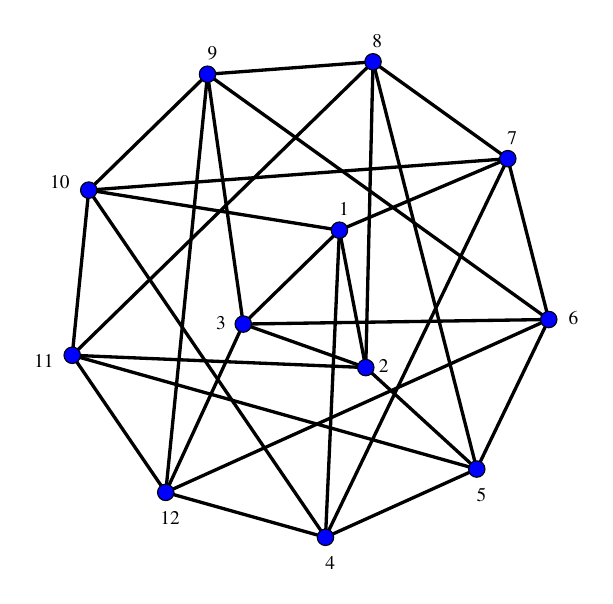
\begin{tikzpicture}[line cap=round,line join=round,>=triangle 45,x=1.0cm,y=1.0cm,scale = .85]
%\clip(-7.216177612974291,1.3842039200742227) rectangle (7.441668823143576,11.680614135410199);
\draw [line width=1.2pt] (-0.6,3.62)-- (2.123558053023431,9.276851992900792);
\draw [line width=1.2pt] (-4.137198504789,8.807096459050374)-- (2.123558053023431,9.276851992900792);
\draw [line width=1.2pt] (-4.137198504789,8.807096459050374)-- (-0.6,3.62);
\draw [line width=1.2pt] (-2.9869038033291604,4.291334665910222)-- (-2.3623537280050293,10.538548456168009);
\draw [line width=1.2pt] (-2.3623537280050293,10.538548456168009)-- (2.735617079568619,6.874065329872934);
\draw [line width=1.2pt] (2.735617079568619,6.874065329872934)-- (-2.9869038033291604,4.291334665910222);
\draw [line width=1.2pt] (-4.383852592928873,6.339879046497543)-- (0.11021214116330502,10.724069405453623);
\draw [line width=1.2pt] (0.11021214116330502,10.724069405453623)-- (1.66,4.64);
\draw [line width=1.2pt] (1.66,4.64)-- (-4.383852592928873,6.339879046497543);
\draw [line width=1.2pt] (-4.383852592928873,6.339879046497543)-- (-4.137198504789,8.807096459050374);
\draw [line width=1.2pt] (-4.137198504789,8.807096459050374)-- (-2.3623537280050293,10.538548456168009);
\draw [line width=1.2pt] (-2.3623537280050293,10.538548456168009)-- (0.11021214116330502,10.724069405453623);
\draw [line width=1.2pt] (0.11021214116330502,10.724069405453623)-- (2.123558053023431,9.276851992900792);
\draw [line width=1.2pt] (2.123558053023431,9.276851992900792)-- (2.735617079568619,6.874065329872934);
\draw [line width=1.2pt] (2.735617079568619,6.874065329872934)-- (1.66,4.64);
\draw [line width=1.2pt] (1.66,4.64)-- (-0.6,3.62);
\draw [line width=1.2pt] (-0.6,3.62)-- (-2.9869038033291604,4.291334665910222);
\draw [line width=1.2pt] (-2.9869038033291604,4.291334665910222)-- (-4.383852592928873,6.339879046497543);
\draw [line width=1.2pt] (-1.8285211049496375,6.806067771006954)-- (-2.3623537280050293,10.538548456168009);
\draw [line width=1.2pt] (-1.8285211049496375,6.806067771006954)-- (2.735617079568619,6.874065329872934);
\draw [line width=1.2pt] (-1.8285211049496375,6.806067771006954)-- (-2.9869038033291604,4.291334665910222);
\draw [line width=1.2pt] (0.001571740633340254,6.156128255753188)-- (-1.8285211049496375,6.806067771006954);
\draw [line width=1.2pt] (-0.3918127028097297,8.208568830238764)-- (-1.8285211049496375,6.806067771006954);
\draw [line width=1.2pt] (-0.3918127028097297,8.208568830238764)-- (0.001571740633340254,6.156128255753188);
\draw [line width=1.2pt] (0.001571740633340254,6.156128255753188)-- (0.11021214116330502,10.724069405453623);
\draw [line width=1.2pt] (0.001571740633340254,6.156128255753188)-- (1.66,4.64);
\draw [line width=1.2pt] (0.001571740633340254,6.156128255753188)-- (-4.383852592928873,6.339879046497543);
\draw [line width=1.2pt] (-0.3918127028097297,8.208568830238764)-- (-4.137198504789,8.807096459050374);
\draw [line width=1.2pt] (-0.3918127028097297,8.208568830238764)-- (2.123558053023431,9.276851992900792);
\draw [line width=1.2pt] (-0.3918127028097297,8.208568830238764)-- (-0.6,3.62);
\begin{scriptsize}
\draw [fill=blue] (-0.6,3.62) circle (3.5pt);
\draw[color=black] (-0.5286420744421019,3.24120280245417) node {$4$};
\draw [fill=blue] (1.66,4.64) circle (3.5pt);
\draw[color=black] (1.7290425574920387,4.250319418242912) node {$5$};
\draw [fill=blue] (2.735617079568619,6.874065329872934) circle (3.5pt);
\draw[color=black] (3.1065738590969693,6.890900378723) node {$6$};
\draw [fill=blue] (2.123558053023431,9.276851992900792) circle (3.5pt);
\draw[color=black] (2.1908416867512948,9.585414382289507) node {$7$};
\draw [fill=blue] (0.11021214116330502,10.724069405453623) circle (3.5pt);
\draw[color=black] (0.17260845517380546,11.039226455883457) node {$8$};
\draw [fill=blue] (-2.3623537280050293,10.538548456168009) circle (3.5pt);
\draw[color=black] (-2.2903202342088935,10.851086069888945) node {$9$};
\draw [fill=blue] (-4.137198504789,8.807096459050374) circle (3.5pt);
\draw[color=black] (-4.569102065429732,8.923615253030252) node {$10$};
\draw [fill=blue] (-4.383852592928873,6.339879046497543) circle (3.5pt);
\draw[color=black] (-4.808553465786383,6.260686563647559) node {$11$};
\draw [fill=blue] (-2.9869038033291604,4.291334665910222) circle (3.5pt);
\draw[color=black] (-2.9231560780086148,3.908245989161983) node {$12$};
\draw [fill=blue] (-1.8285211049496375,6.806067771006954) circle (3.5pt);
\draw[color=black] (-2.1601064191334512,6.822485692906814) node {$3$};
\draw [fill=blue] (0.001571740633340254,6.156128255753188) circle (3.5pt);
\draw[color=black] (0.26998642644952634,6.172546177653048) node {$2$};
\draw [fill=blue] (-0.3918127028097297,8.208568830238764) circle (3.5pt);
\draw[color=black] (-0.32339801699354365,8.524986752138625) node {$1$};
\end{scriptsize}
\end{tikzpicture}
\end{minipage}&
%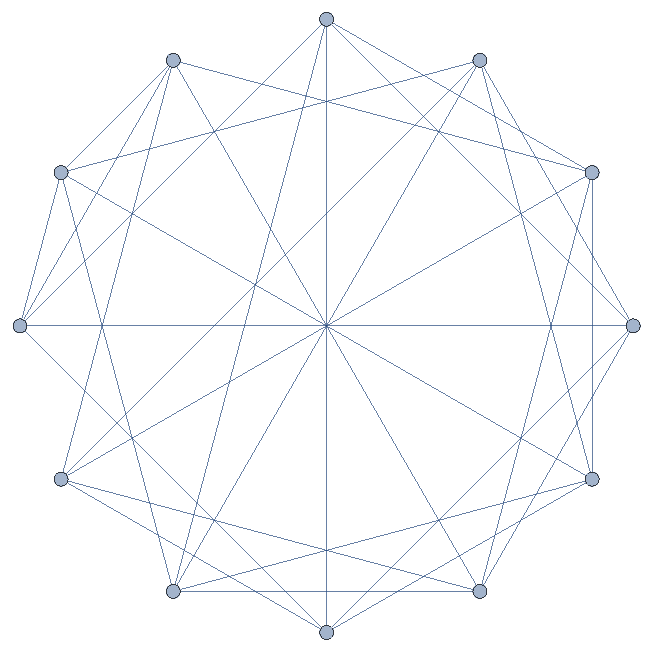
\includegraphics[scale=.7]{ex1_0.pdf}

\begin{minipage}[b]{.47\textwidth}

 $\left[\begin{array}{lll || lll | lll | lll}
0 & 1 & 1 & 1 & 0 & 0 & 1 & 0 &  0 & 1 & 0 & 0\\
1 & 0 & 1 & 0 & 1 & 0 & 0 & 1 & 0 &  0 &  1 &  0\\
1 & 1 & 0 & 0 & 0 & 1 & 0 & 0 & 1 & 0 & 0 & 1\\\hline \hline 
1 & 0 & 0 & 0 & 1 & 0 & 1 & 0 & 0 & 1 & 0 & 1\\
0 & 1 & 0 & 1 & 0 & 1 & 0 & 1 & 0 & 0 & 1 &0\\
0 & 0 & 1 & 0 & 1 & 0 & 1 & 0 & 1 & 0 & 0 & 1\\\hline
1 & 0 & 0 & 1 &0 & 1 & 0 & 1 & 0 & 1 & 0 & 0\\
0 & 1 & 0 & 0 & 1 & 0 & 1 & 0 & 1 & 0 & 1 & 0\\
0 & 0 & 1 & 0 & 0 & 1 & 0 & 1 & 0 & 1 & 0 & 1\\\hline
1 & 0 & 0 & 1 & 0 & 0 & 1 & 0 & 1 & 0 & 1 & 0\\
0 & 1 & 0 & 0 & 1 & 0 & 0 & 1 & 0 & 1 & 0 & 1\\
0 & 0 & 1 & 1 & 0 & 1 & 0 & 0 & 1 & 0 & 1 & 0
\end{array}\right]$
\vspace{.5cm}

\end{minipage}
\end{tabular}
\caption{The graph $G$ on 12 vertices with automorphism $\phi=(1,2,3)(4,5,6,7,8,9,10,11,12)$, and its adjacency matrix.}
\end{figure}

We attempt to follow the recursive method of equitable decompositions for separable automorphisms \cite{FSSW} by first forming a new automorphism $\psi=\phi^3=(4,7,10)(5,8,11)(6,9,12)$. The first decomposition gives a direct sum of smaller matrices with the following associated digraphs.

\begin{figure}[h!]
\begin{center}
$\left[\begin{array}{lll | lll }
0 & 1 & 1 & 3 & 0 & 0 \\
1 & 0 & 1 & 0 & 3 & 0\\
1 & 1 & 0 & 0 & 0 & 3 \\\hline 
1 & 0 & 0 & 2 & 1 & 1 \\
0 & 1 & 0 & 1 & 2 & 1 \\
0 & 0 & 1 & 1 & 1 & 2 
\end{array}\right] \oplus 
\left[\begin{array}{lll }
\w +\w^2& 1 & \w^2  \\
1 & \w + \w^2 & 1 \\
\w & 1 & \w + \w^2  \\
\end{array}\right]\oplus 
\left[\begin{array}{lll }
\w +\w^2& 1 & \w  \\
1 & \w + \w^2 & 1 \\
\w^2 & 1 & \w + \w^2  \\
\end{array}\right]$ \\[2mm]


\begin{tabular}{c}
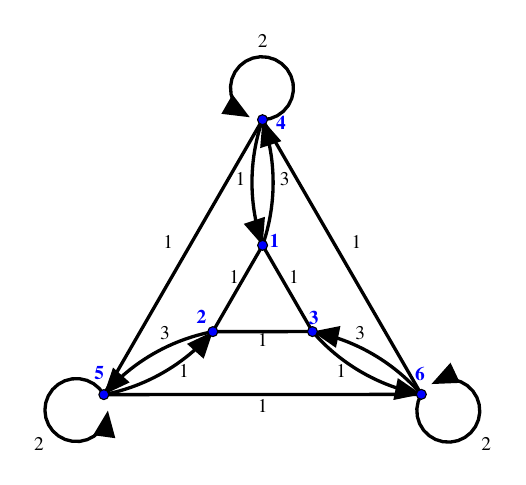
\begin{tikzpicture}[line cap=round,line join=round,>=triangle 45,x=1.0cm,y=1.0cm, scale = .4]
\draw [line width=1.2pt] (3.,2.)-- (1.42,-0.74);
\draw [line width=1.2pt] (1.42,-0.74)-- (4.582909606369362,-0.738320137979414);
\draw [line width=1.2pt] (4.582909606369362,-0.738320137979414)-- (3.,2.);
\draw [->, shift={(8.746530801304676,3.9975601362061384)},line width=1.2pt]  plot[domain=2.808109490764957:3.47613804206866,variable=\t]({1.*6.083819749803839*cos(\t r)+0.*6.083819749803839*sin(\t r)},{0.*6.083819749803839*cos(\t r)+1.*6.083819749803839*sin(\t r)});
\draw [->,shift={(-2.7619038286835558,3.9914478583805644)},line width=1.2pt]  plot[domain=-0.3327703910467745:0.33383261670080516,variable=\t]({1.*6.096343191097985*cos(\t r)+0.*6.096343191097985*sin(\t r)},{0.*6.096343191097985*cos(\t r)+1.*6.096343191097985*sin(\t r)});
\draw [->, shift={(2.574873153942068,-6.730834430650846)},line width=1.2pt]  plot[domain=1.7612336156607167:2.4286188147797056,variable=\t]({1.*6.1011334338111105*cos(\t r)+0.*6.1011334338111105*sin(\t r)},{0.*6.1011334338111105*cos(\t r)+1.*6.1011334338111105*sin(\t r)});
\draw [->,shift={(-3.190222966731918,3.2423685501799246)},line width=1.2pt]  plot[domain=4.902310947532458:5.570726790087551,variable=\t]({1.*6.09207805863029*cos(\t r)+0.*6.09207805863029*sin(\t r)},{0.*6.09207805863029*cos(\t r)+1.*6.09207805863029*sin(\t r)});
\draw [->,shift={(3.4409228960059806,-6.713365807470568)},line width=1.2pt]  plot[domain=0.7135095119397563:1.3819478161074714,variable=\t]({1.*6.083198533596579*cos(\t r)+0.*6.083198533596579*sin(\t r)},{0.*6.083198533596579*cos(\t r)+1.*6.083198533596579*sin(\t r)});
\draw [->,shift={(9.177088828763083,3.23416245566517)},line width=1.2pt]  plot[domain=3.854546186837524:4.524096448389289,variable=\t]({1.*6.073475173595705*cos(\t r)+0.*6.073475173595705*sin(\t r)},{0.*6.073475173595705*cos(\t r)+1.*6.073475173595705*sin(\t r)});
\draw [->,shift={(2.9803003568273967,6.988860475994255)},line width=1.2pt]  %(0,0) --
  plot[domain=-1.5532143950535158:4.314098663792105,variable=\t]({1.*1.*cos(\t r)+0.*1.*sin(\t r)},{0.*1.*cos(\t r)+1.*1.*sin(\t r)}) ;%-- cycle ;
\draw [->,shift={(8.89586008462023,-3.249577222650493)},line width=1.2pt]    plot[domain=-3.6856496994623047:2.1335046414728542,variable=\t]({1.*1.*cos(\t r)+0.*1.*sin(\t r)},{0.*1.*cos(\t r)+1.*1.*sin(\t r)})  ;
\draw [->,shift={(-2.911791543957258,-3.2303056150093457)},line width=1.2pt]   plot[domain=0.512248008742023:6.265411724401079,variable=\t]({1.*1.*cos(\t r)+0.*1.*sin(\t r)},{0.*1.*cos(\t r)+1.*1.*sin(\t r)});
\draw [line width=1.2pt] (2.9978813827489854,5.9890150341745985)-- (-2.0401466673309936,-2.7401676660080625);
\draw [line width=1.2pt] (-2.0401466673309936,-2.7401676660080625)-- (8.040244329607463,-2.7319657083137923);
\draw [line width=1.2pt] (8.040244329607463,-2.7319657083137923)-- (2.9978813827489854,5.9890150341745985);
\begin{scriptsize}
\draw [fill=blue] (3.,2.) circle (4.5pt);
\draw[color=blue] (3.3797862649889464,2.1344492655878913) node {${\bf 1}$};
\draw [fill=blue] (1.42,-0.74) circle (4.5pt);
\draw[color=blue] (1.0607506144093768,-0.2652055658528048) node {${\bf 2}$};
\draw [fill=blue] (4.582909606369362,-0.738320137979414) circle (4.5pt);
\draw[color=blue] (4.621528751385895,-0.291008305975823) node {${\bf3}$};
\draw [fill=blue] (2.9978813827489854,5.9890150341745985) circle (4.5pt);
\draw[color=blue] (3.5797862649889464,5.901649323548554) node {${\bf4}$};
\draw [fill=blue] (-2.0401466673309936,-2.7401676660080625) circle (4.5pt);
\draw[color=blue] (-2.1903946410909225,-2.045594634341063) node {${\bf5}$};
\draw [fill=blue] (8.040244329607463,-2.7319657083137923) circle (4.5pt);
\draw[color=blue] (8,-2.0972001145870998) node {${\bf6}$};

\draw[color=black] (5.9797862649889464,2.101649323548554) node {$1$};
\draw[color=black] (0,2.101649323548554) node {$1$};
\draw[color=black] (3,-3.101649323548554) node {$1$};
\draw[color=black] (10.1,-4.301649323548554) node {$2$};
\draw[color=black] (-4.1,-4.301649323548554) node {$2$};
\draw[color=black] (3,8.5) node {$2$};
\draw[color=black] (3.7,4.1) node {$3$};
\draw[color=black] (2.3,4.1) node {$1$};
\draw[color=black] (-.1,-.8) node {$3$};
\draw[color=black] (0.5,-2) node {$1$};
\draw[color=black] (6.1,-.8) node {$3$};
\draw[color=black] (5.5,-2) node {$1$};
\draw[color=black] (2.1,1) node {$1$};
\draw[color=black] (4,1) node {$1$};
\draw[color=black] (3,-1) node {$1$};
\end{scriptsize}
\end{tikzpicture}


\hspace*{-.7cm}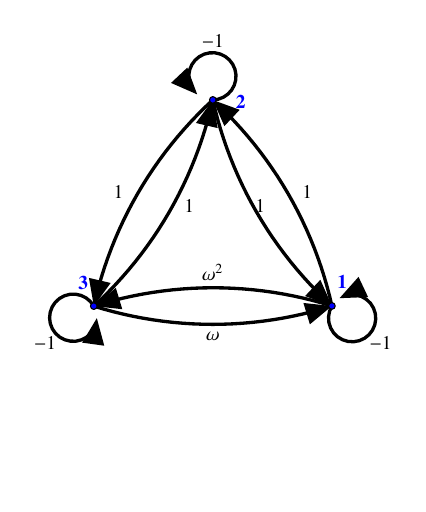
\begin{tikzpicture}[line cap=round,line join=round,>=triangle 45,x=1.0cm,y=1.0cm,scale = .3]
%\clip(-8.537868711353411,-7.65769061109753) rectangle (12.439759008660426,8.778654847265086);
\draw [->, shift={(3.0130847985281797,-18.75756462853538)},line width=1.2pt]  plot[domain=1.2668226187643103:1.8763973439024366,variable=\t]({1.*16.79559923619067*cos(\t r)+0.*16.79559923619067*sin(\t r)},{0.*16.79559923619067*cos(\t r)+1.*16.79559923619067*sin(\t r)});
\draw [->, shift={(19.37392598872407,9.63923476036045)},line width=1.2pt]  plot[domain=3.3609073531733613:3.970731049757719,variable=\t]({1.*16.777930175868597*cos(\t r)+0.*16.777930175868597*sin(\t r)},{0.*16.777930175868597*cos(\t r)+1.*16.777930175868597*sin(\t r)});
\draw [->, shift={(-8.333612517864772,-6.380920499656055)},line width=1.2pt]  plot[domain=0.2192694750466929:0.8291836207048014,variable=\t]({1.*16.775519638174345*cos(\t r)+0.*16.775519638174345*sin(\t r)},{0.*16.775519638174345*cos(\t r)+1.*16.775519638174345*sin(\t r)});
\draw [->, shift={(14.35091983175103,-6.3818000228558365)},line width=1.2pt]  plot[domain=2.313319799013006:2.9229717803830764,variable=\t]({1.*16.790728012798304*cos(\t r)+0.*16.790728012798304*sin(\t r)},{0.*16.790728012798304*cos(\t r)+1.*16.790728012798304*sin(\t r)});
\draw [->, shift={(-13.389609820737382,9.628583917256625)},line width=1.2pt]  plot[domain=5.454838648429755:6.064638238145913,variable=\t]({1.*16.786790330466452*cos(\t r)+0.*16.786790330466452*sin(\t r)},{0.*16.786790330466452*cos(\t r)+1.*16.786790330466452*sin(\t r)});
\draw [->, shift={(2.9940079090559673,13.282142090759644)},line width=1.2pt]  plot[domain=4.407959240767685:5.017651628291141,variable=\t]({1.*16.794556327595302*cos(\t r)+0.*16.794556327595302*sin(\t r)},{0.*16.794556327595302*cos(\t r)+1.*16.794556327595302*sin(\t r)});
\draw [shift={(2.9803003568273967,6.988860475994255)},line width=1.2pt,->]  plot[domain=-1.5532143950535158:4.014098663792105,variable=\t]({1.*1.*cos(\t r)+0.*1.*sin(\t r)},{0.*1.*cos(\t r)+1.*1.*sin(\t r)}) ;
\draw [shift={(8.89586008462023,-3.249577222650493)},line width=1.2pt,->]    plot[domain=-3.6856496994623047:2.1335046414728542,variable=\t]({1.*1.*cos(\t r)+0.*1.*sin(\t r)},{0.*1.*cos(\t r)+1.*1.*sin(\t r)})  ;
\draw [shift={(-2.911791543957258,-3.2303056150093457)},line width=1.2pt, ->]    plot[domain=0.512248008742023:6.265411724401079,variable=\t]({1.*1.*cos(\t r)+0.*1.*sin(\t r)},{0.*1.*cos(\t r)+1.*1.*sin(\t r)})  ;
\begin{scriptsize}
\draw [fill=blue] (2.9978813827489854,5.9890150341745985) circle (4pt);
\draw[color=blue] (4.1797862649889464,5.901649323548554) node {${\bf 2}$};
\draw [fill=blue] (-2.0401466673309936,-2.7401676660080625) circle (4pt);
\draw[color=blue] (-2.4903946410909225,-1.745594634341063) node {${\bf 3}$};
\draw [fill=blue] (8.040244329607463,-2.7319657083137923) circle (4pt);
\draw[color=blue] (8.472674006886195,-1.6972001145870998) node {${\bf 1}$};

\draw[color=black] (-1,2.101649323548554) node {$1$};
\draw[color=black] (3,-4) node {$\w$};
\draw[color=black] (10.1,-4.301649323548554) node {$-1$};
\draw[color=black] (-4.1,-4.301649323548554) node {$-1$};
\draw[color=black] (3,8.5) node {$-1$};
%\draw[color=black] (10.1,-4.301649323548554) node {$\w + \w^2$};
%\draw[color=black] (-4.1,-4.301649323548554) node {$\w + \w^2$};
%\draw[color=black] (3,8.5) node {$\w + \w^2$};
\draw[color=black] (3,-1.3) node {$\w^2$};
\draw[color=black] (2,1.5) node {$1$};
\draw[color=black] (5,1.5) node {$1$};
\draw[color=black] (7,2.101649323548554) node {$1$};
\draw[color=black] (3,-10) node {$$};


\end{scriptsize}
\end{tikzpicture}


\hspace*{-.7cm}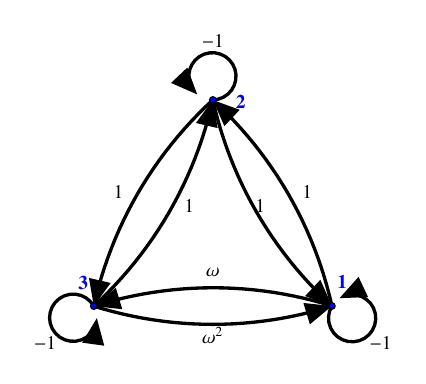
\begin{tikzpicture}[line cap=round,line join=round,>=triangle 45,x=1.0cm,y=1.0cm,scale = .3]
%\clip(-8.537868711353411,-7.65769061109753) rectangle (12.439759008660426,8.778654847265086);
\draw [->, shift={(3.0130847985281797,-18.75756462853538)},line width=1.2pt]  plot[domain=1.2668226187643103:1.8763973439024366,variable=\t]({1.*16.79559923619067*cos(\t r)+0.*16.79559923619067*sin(\t r)},{0.*16.79559923619067*cos(\t r)+1.*16.79559923619067*sin(\t r)});
\draw [->, shift={(19.37392598872407,9.63923476036045)},line width=1.2pt]  plot[domain=3.3609073531733613:3.970731049757719,variable=\t]({1.*16.777930175868597*cos(\t r)+0.*16.777930175868597*sin(\t r)},{0.*16.777930175868597*cos(\t r)+1.*16.777930175868597*sin(\t r)});
\draw [->, shift={(-8.333612517864772,-6.380920499656055)},line width=1.2pt]  plot[domain=0.2192694750466929:0.8291836207048014,variable=\t]({1.*16.775519638174345*cos(\t r)+0.*16.775519638174345*sin(\t r)},{0.*16.775519638174345*cos(\t r)+1.*16.775519638174345*sin(\t r)});
\draw [->, shift={(14.35091983175103,-6.3818000228558365)},line width=1.2pt]  plot[domain=2.313319799013006:2.9229717803830764,variable=\t]({1.*16.790728012798304*cos(\t r)+0.*16.790728012798304*sin(\t r)},{0.*16.790728012798304*cos(\t r)+1.*16.790728012798304*sin(\t r)});
\draw [->, shift={(-13.389609820737382,9.628583917256625)},line width=1.2pt]  plot[domain=5.454838648429755:6.064638238145913,variable=\t]({1.*16.786790330466452*cos(\t r)+0.*16.786790330466452*sin(\t r)},{0.*16.786790330466452*cos(\t r)+1.*16.786790330466452*sin(\t r)});
\draw [->, shift={(2.9940079090559673,13.282142090759644)},line width=1.2pt]  plot[domain=4.407959240767685:5.017651628291141,variable=\t]({1.*16.794556327595302*cos(\t r)+0.*16.794556327595302*sin(\t r)},{0.*16.794556327595302*cos(\t r)+1.*16.794556327595302*sin(\t r)});
\draw [shift={(2.9803003568273967,6.988860475994255)},line width=1.2pt,->]  plot[domain=-1.5532143950535158:4.014098663792105,variable=\t]({1.*1.*cos(\t r)+0.*1.*sin(\t r)},{0.*1.*cos(\t r)+1.*1.*sin(\t r)}) ;
\draw [shift={(8.89586008462023,-3.249577222650493)},line width=1.2pt,->]    plot[domain=-3.6856496994623047:2.1335046414728542,variable=\t]({1.*1.*cos(\t r)+0.*1.*sin(\t r)},{0.*1.*cos(\t r)+1.*1.*sin(\t r)})  ;
\draw [shift={(-2.911791543957258,-3.2303056150093457)},line width=1.2pt, ->]    plot[domain=0.512248008742023:6.265411724401079,variable=\t]({1.*1.*cos(\t r)+0.*1.*sin(\t r)},{0.*1.*cos(\t r)+1.*1.*sin(\t r)})  ;
\begin{scriptsize}
\draw [fill=blue] (2.9978813827489854,5.9890150341745985) circle (4pt);
\draw[color=blue] (4.1797862649889464,5.901649323548554) node {${\bf 2}$};
\draw [fill=blue] (-2.0401466673309936,-2.7401676660080625) circle (4pt);
\draw[color=blue] (-2.4903946410909225,-1.745594634341063) node {${\bf 3}$};
\draw [fill=blue] (8.040244329607463,-2.7319657083137923) circle (4pt);
\draw[color=blue] (8.472674006886195,-1.6972001145870998) node {${\bf 1}$};

\draw[color=black] (-1,2.101649323548554) node {$1$};
\draw[color=black] (3,-4) node {$\w^2$};
\draw[color=black] (10.1,-4.301649323548554) node {$-1$};
\draw[color=black] (-4.1,-4.301649323548554) node {$-1$};
\draw[color=black] (3,8.5) node {$-1$};
%\draw[color=black] (10.1,-4.301649323548554) node {$\w + \w^2$};
%\draw[color=black] (-4.1,-4.301649323548554) node {$\w + \w^2$};
%\draw[color=black] (3,8.5) node {$\w + \w^2$};
\draw[color=black] (3,-1.3) node {$\w$};
\draw[color=black] (2,1.5) node {$1$};
\draw[color=black] (5,1.5) node {$1$};
\draw[color=black] (7,2.101649323548554) node {$1$};
\end{scriptsize}
\end{tikzpicture} \end{tabular}
\end{center}
\caption{The decomposition of the graph $G$ on 12 vertices using the basic  automorphism $\psi=(4,7, 10), (5, 8, 11), (6, 9, 12)$.}
\end{figure}


%\begin{center}
%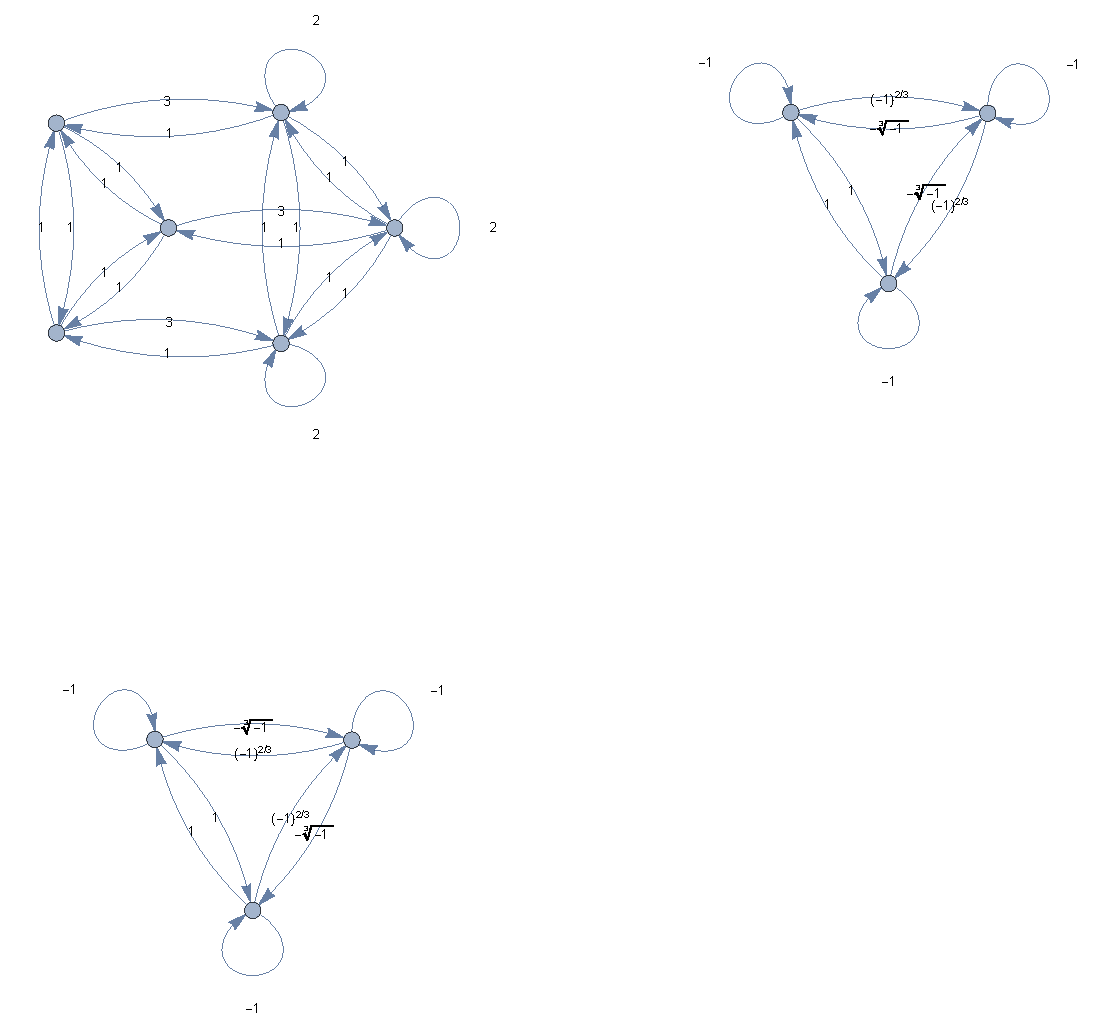
\includegraphics[scale=.5]{ex1_1.pdf}
%\end{center}
While there is an automorphism of order three which acts on the first ``piece'' of the decomposed matrix, there is no automorphism permuting all of the vertices of $G$ as $\phi$ does.  Thus, if we continue the recursive process in this example, we fail to account for part of the symmetry found in $\phi$.   This decomposition was done using the transversal $\cT_0=\{4,8,12\}$ (See \cite{BFW, FSSW} for details). One may wonder if a different choice of semi-transversal could give better results. However, simple computations demonstrate that any choice of transversal yields a similarly unsatisfying conclusion. Thus we conclude that the methods contained in \cite{BFW} and \cite{FSSW} cannot be used to completely decompose examples like this.
\end{example}

\marginpar{\dscomm{we need to make a comment about the $N=1$ case.  It is a basic automorphism}}
\section{Equitable Decompositions using Arbitrary Automorphisms}
In this section we give a method for decomposing a graph using any automorphism.  First, however, we will need the following Lemma. 
\begin{lem}\label{lem:Dallas}
Let $M$ be the $(f + rp^N) \times (f + rp^N)$ block matrix
\begin{equation}\label{eq:defineM}
M = \left[\begin{array}{llllll}
F & H & H & H & \cdots & H \\
L &  \\
L &  \\
L &  & C \\
\vdots &  \\
L &  \\
\end{array}\right],
\end{equation}
where $F$ is $f \times f$, $H$ is $f \times rp^{N-1}$,  $L$ is $rp^{N-1} \times f$, and $C$ is $rp^N \times rp^N$.  Suppose that the matrix $C$ can be partitioned in two ways:
\[
C =  \left[\begin{array}{lllll}
 C_0 & C_1 & C_2 & \cdots & C_{p^N-1} \\
 C_{p^N-1} & C_0 & C_1 & \cdots & C_{p^N-2} \\
 C_{p^N-2} & C_{p^N-1} & C_0 & \cdots & C_{p^N-3} \\
 \vdots & \vdots & \vdots & & \vdots \\
 C_1 & C_2 & C_3 & \cdots & C_0 \\
\end{array}\right] =
\left[\begin{array}{lllll}
 D_0 & D_1 & D_2 & \cdots & D_{p-1} \\
 D_{p-1} & D_0 & D_1 & \cdots & D_{p-2} \\
 D_{p-2} & D_{p-1} & D_0 & \cdots & D_{p-3} \\
 \vdots & \vdots & \vdots & & \vdots \\
 D_1 & D_2 & D_3 & \cdots & D_0 \\
\end{array}\right]
\]
with each $D_i$ block of size $rp^{N-1} \times rp^{N-1}$, and each $C_j$ of size $r \times r$.
  Then there exists an $(f + rp^{N}) \times (f  +rp^N)$ invertible matrix $T$ such that
\begin{equation}\label{eq:sim_decomp}
T^{-1} M T = \left[\begin{array}{rr} F & pH \\ L & B_0 \end{array}\right]
\oplus B_1 \oplus B_2 \oplus \cdots \oplus B_{p^N-p^{N-1}},
\end{equation}
with
\[
B_0 = \sum_{m=0}^{p-1} D_m, \ \text{and }
B_j = \sum_{m=0}^{p^N-1} \omega^{\gamma_j m}C_m \ \ \text{for} \ \ j = 1,2, \ldots, p^N-p^{N-1}, 
\]
where  $\gamma_j$ are elements of $\{1,2,\dots ,p^N-1\}$ which are not multiples of $p$. Consequently,
\[
\sigma(M) = \sigma\left(\left[\begin{array}{rr} F & pH \\ L & B_0 \end{array}\right] \right)
\cup \sigma(B_1) \cup \sigma(B_2) \cup \cdots \cup \sigma(B_{p^N-p^{N-1}}).
\]
\end{lem}

\begin{proof}
Before we begin let us establish some useful identities  involving roots of unity. Recall that if $\omega = e^{\frac{2\pi i }{p^N}}$, $0< \gamma, \ \gamma' < p^N$ are distinct integers, both relatively prime to $p$, and $a$ is any integer,  then 

\begin{equation}\label{eq:rtsofunity}
\sum\limits_{m=0}^{p-1}\omega^{\gamma_b (m p^{N-1}+a)}=0, \text{ and } \sum\limits_{m=0}^{p^{N}-1}\omega^{m(\gamma_a-\gamma_b)}=0.
\end{equation} 
%\begin{equation}\label{eq2}
%\sum\limits_{m=0}^{p^{N}-1}\omega^{m(\gamma_a-\gamma_b)}=0
%\end{equation} whenever $a\neq b$.
  Let $S$ be the $rp^N \times rp^{N-1}(p-1)$ block matrix written below in $r \times r$ blocks: 
 \[
S = \left[\begin{array}{llll}
 I & I & \ldots & I \\
 \omega^{\gamma_1} I & \omega^{\gamma_2} I & \ldots & \omega^{\gamma_\rho} I \\
 \omega^{2\gamma_1} I & \omega^{2\gamma_2} I & \ldots & ^{2\gamma_\rho} I \\
\vdots  & \vdots & & \vdots \\
 \omega^{(p^N-1)\gamma_1} I & \omega^{(p^N-1)\gamma_2} I & \ldots & \omega^{(p^N-1)\gamma_\rho} I
 \end{array}\right],
\]
where $\omega = e^{2\pi i /p^N}$, and $\omega^{\gamma_1}, \omega^{\gamma_2}, \ldots, \omega^{\gamma_\rho}$ are  the $p^N - p^{N-1}$ generators of the cyclic group or $p^N$-roots of unity. We let $T$ be the block matrix
\[
T = \left[\begin{array}{c | c | c}
I_f & 0 & 0 \\\hline
 & I_{rp^{N-1}} &  \\
0 & I_{rp^{N-1}} & S \\
&\vdots &  \\
 & I_{rp^{N-1}} &  \\
\end{array}\right].
\]
%Now the first thing we need to show is the form of $T^{-1}$, which we can prove by demonstrating that $T^{-1}T=I$. 
Let $R=\left[\begin{array}{l l l l}I_{rp^{N-1}}& I_{rp^{N-1}}&\cdots& I_{rp^{N-1}}\end{array}\right]$ and consider the product
\[
 \left[\begin{array}{cc  }
I_f & 0 \\[1mm]
0 & \frac{1}{p}R \\[1mm]
 0 & \frac{1}{p^N}S^*   \\
\end{array}\right]
 \left[\begin{array}{ccc}
I_f & 0 & 0 \\
 0& R^T & S \\
\end{array}\right]
=\left[\begin{array}{ccc}
I_f & 0 & 0 \\[1mm]
 0 & \frac{1}{p}RR^T% I_{rp^{N-1}} 
 & \frac{1}{p}RS \\[1mm]
0 & \frac{1}{p^N}S^*R^T & \frac{1}{p^N}S^*S \\

\end{array}\right].
\]
%We can calculate each block of the matrix, starting with $RS$. For notational simplicity, we write $RS=\left[G_0 \quad G_1 \quad \cdots \quad G_{p-1}\right]$, where each $G_i$ is a $rp^{N-1}\times rp^{N-1}$ matrix.
%with the form
%$$
%G_i=\left[\begin{array}{llll}
%I\sum\limits_{m=0}^{p-1}\omega^{\gamma_{1+i}mp^{N-1}}&I\sum\limits_{m=0}^{p-1}\omega^{\gamma_{2+i}mp^{N-1}}&\cdots&I\sum\limits_{m=0}^{p-1}\omega^{\gamma_{p^{N-1}+i}mp^{N-1}}\\
%I\sum\limits_{m=0}^{p-1}\omega^{\gamma_{1+i}(mp^{N-1}+1)}&I\sum\limits_{m=0}^{p-1}\omega^{\gamma_{2+i}(mp^{N-1}+1)}&\cdots&I\sum\limits_{m=0}^{p-1}\omega^{\gamma_{p^{N-1}+i}(mp^{N-1}+1)}\\\vdots&\vdots&&\vdots
%\\
%I\sum\limits_{m=0}^{p-1}\omega^{\gamma_{1+i}(mp^{N-1}+p^{N-1}-1)}&I\sum\limits_{m=0}^{p-1}\omega^{\gamma_{2+i}(mp^{N-1}+p^{N-1}-1)}&\cdots&I\sum\limits_{m=0}^{p-1}\omega^{\gamma_{p^{N-1}+i}(mp^{N-1}+p^{N-1}-1)}
%\end{array}\right]
%$$
%If we think of each $G_i$ as block matrix with $r\times r$ blocks,
The matrix $RS$ is comprised of $p$ $rp^{N-1} \times rp^{N-1}$ blocks, each of the form
\[
 %\left[G_i\right]_{a,b}=
 I_r\sum\limits_{m=0}^{p-1}\omega^{\gamma_{b}(mp^{N-1}+a-1)}=0. %\qquad 1\leq a,b \leq p^{N-1} 
 \]
%Each the matrix entry in $G_i$ contains a sum in the form of Eq. \ref{eq1} thus we can conclude that $RS=\left[ 0\right]$.
Similarly, $S^*R^T=0$. 

Next we consider $S^*S$ as a block matrix with $r\times r$ blocks, the $ (a,b)^{th} $ block has the form 
\[
%\left[ S^*S\right]_{a,b}=p^N
I_r\sum\limits_{m=0}^{p^{N}-1}\omega^{m(\gamma_b-\gamma_a)} %\qquad 1\leq a,b \leq p^N-p^{N-1}.
=\left\{\begin{array}{cl}
p^NI_r & \text{if} \ a=b\\
0_r & \text{if} \ a \neq b
\end{array}\right.
\]
So, $S^*S=p^N I$, and therefore 
\[
T^{-1}= \left[\begin{array}{cc  }
I_f & 0 \\[1mm]
0 & \frac{1}{p}R \\[1mm]
 0 & \frac{1}{p^N}S^*   \\
\end{array}\right].
\]

Next we show that performing a similarity transformation using $T$ gives the equitable decomposition in Equation \ref{eq:sim_decomp}.
Let $M$ be the matrix given in Equation \ref{eq:defineM}.  Then with $P = \left[ H \quad H \cdots H\right]$ and
$Q = [ L^T \quad L^T \cdots L^T]^T$,
\[
T^{-1}MT = \left[\begin{array}{cc  }
I_f & 0 \\[1mm]
0 & \frac{1}{p}R \\[1mm]
 0 & \frac{1}{p^N}S^*   \\
\end{array}\right]
\left[\begin{array}{rr} F & P \\ Q & C \end{array}\right]
 \left[\begin{array}{ccc}
I_f & 0 & 0 \\
 0& R^T & S \\
\end{array}\right] 
=\left[\begin{array}{ccc} 
F & PR^T & PS \\[1mm]
\frac{1}{p}RQ  & \frac{1}{p}RCR^T & \frac{1}{p}RCS\\[1mm]
 \frac{1}{p^N}S^*Q & \frac{1}{p^N} S^*CR^T & \frac{1}{p^N}S^*CS \end{array}\right].\label{blocks}
\]
%\begin{align}
%T^{-1}MT &= \left[\begin{array}{l | l  }
%I_f & 0 \\\hline
%0 & (1/p)R \\\hline
% 0 & (1/p^N)S^*   \\
%\end{array}\right]
%\left[\begin{array}{rr} F & P \\ Q & C \end{array}\right]
% \left[\begin{array}{l | l | l}
%I_f & 0 & 0 \\\hline
% 0& R^T & S \\
%\end{array}\right] \nonumber \\
%&=\left[\begin{array}{rrr} I_f & PR^T & PS \\(1/p)RQ  & (1/p)RCR^T & (1/p)RCS\\ (1/p^N)S^*Q & (1/p^N) S^*CR^T & (1/p^N)S^*CS \end{array}\right].\label{blocks}
%\end{align}
It is straightforward to verify that 
\[
PR^T=pH, \quad RQ=pL, \quad \text{and} \quad RCR^T=p\sum_{m=0}^{p-1}{D_m}=pB_0.
\]
To show that $PS = 0$, we break $H$ into $f \times r$ blocks $H_i$ and observe that $H_I = H_{i + p^{N-2}}$. The $k$th $f \times r$ block in the product $PS$ is given by 
\[ \sum_{i=0}^{p^{N-1}-1}H_i\sum_{m=0}^{p-1}\omega^{\gamma_k (mp^{N-1}+i)} =0,
\]
as in Equation \ref{eq:rtsofunity}. A similar calculation shows that $S^*Q=0$. Next we consider the matrix product $RCS$.
%$$RCS=R\left[\begin{array}{lllll}
% C_0 & C_1 & C_2 & \cdots & C_{p^N-1} \\
% C_{p^N-1} & C_0 & C_1 & \cdots & C_{p^N-2} \\
% C_{p^N-2} & C_{p^N-1} & C_0 & \cdots & C_{p^N-3} \\
% \vdots & \vdots & \vdots & & \vdots \\
% C_1 & C_2 & C_3 & \cdots & C_0 \\
%\end{array}\right] \left[\begin{array}{llll}
% I & I & \ldots & I \\
% \omega^{\gamma_1} I & \omega^{\gamma_2} I & \ldots & \omega^{\gamma_\rho} I \\
% \omega^{2\gamma_1} I & \omega^{2\gamma_2} I & \ldots & ^{2\gamma_\rho} I \\
%\vdots  & \vdots & & \vdots \\
% \omega^{(p^N-1)\gamma_1} I & \omega^{(p^N-1)\gamma_2} I & \ldots & \omega^{(p^N-1)\gamma_\rho} I
% \end{array}\right]$$
% $$=R\left[ {\begin{matrix}   {\sum\limits_{m = 0}^{{p^N} - 1} {{C_m}{\omega ^{m{\gamma _1}}}} } & {\sum\limits_{m = 0}^{{p^N} - 1} {{C_m}{\omega ^{m{\gamma _2}}}} } &  \cdots  & {\sum\limits_{m = 0}^{{p^N} - 1} {{C_m}{\omega ^{m{\gamma _\rho }}}} }  \\
%   {\sum\limits_{m = 0}^{{p^N} - 1} {{C_m}{\omega ^{(m + 1){\gamma _1}}}} } & {\sum\limits_{m = 0}^{{p^N} - 1} {{C_m}{\omega ^{(m + 1){\gamma _2}}}} } &  \cdots  & {\sum\limits_{m = 0}^{{p^N} - 1} {{C_m}{\omega ^{(m + 1){\gamma _\rho }}}} }  \\
%    \vdots  &  \vdots  &  \ddots  &  \vdots   \\
%   {\sum\limits_{m = 0}^{{p^N} - 1} {{C_m}{\omega ^{(m + {p^N} - 1){\gamma _1}}}} } & {\sum\limits_{m = 0}^{{p^N} - 1} {{C_m}{\omega ^{(m + {p^N} - 1){\gamma _2}}}} } &  \cdots  & {\sum\limits_{m = 0}^{{p^N} - 1} {{C_m}{\omega ^{(m + {p^N} - 1){\gamma _\rho }}}} }  \\
% \end{matrix} } \right]
% $$
 %$$
 %=\left[ {\begin{array}{rrrr}   {\sum\limits_{m = 0}^{{p^N} - 1} {C_m}{\omega^{m\gamma_1}\sum\limits_{j=0}^{p-1}{\omega ^{\gamma _1(jp^{N-1})}}} } & {\sum\limits_{m = 0}^{{p^N} - 1} {C_m}{\omega^{m\gamma_2}\sum\limits_{j=0}^{p-1}{\omega ^{\gamma _2(jp^{N-1})}}} } &  \cdots  &  {\sum\limits_{m = 0}^{{p^N} - 1} {C_m}{\omega^{m\gamma_{\rho}}\sum\limits_{j=0}^{p-1}{\omega ^{\gamma _{\rho}(jp^{N-1})}}} }  \\
%    {\sum\limits_{m = 0}^{{p^N} - 1} {C_m}{\omega^{(m+1)\gamma_1}\sum\limits_{j=0}^{p-1}{\omega ^{\gamma _1(jp^{N-1})}}} } & {\sum\limits_{m = 0}^{{p^N} - 1} {C_m}{\omega^{(m+1)\gamma_2}\sum\limits_{j=0}^{p-1}{\omega ^{\gamma _2(jp^{N-1})}}} } &  \cdots  & {\sum\limits_{m = 0}^{{p^N} - 1} {C_m}{\omega^{(m+1)\gamma_{\rho}}\sum\limits_{j=0}^{p-1}{\omega ^{\gamma _{\rho}(jp^{N-1})}}} }  \\
%    \vdots  &  \vdots  &  \ddots  &  \vdots   \\
%   {\sum\limits_{m = 0}^{{p^N} - 1} {C_m}{\omega^{(m+p^N-1)\gamma_1}\sum\limits_{j=0}^{p-1}{\omega ^{\gamma _1(jp^{N-1})}}} } &  {\sum\limits_{m = 0}^{{p^N} - 1} {C_m}{\omega^{(m+p^N-1)\gamma_2}\sum\limits_{j=0}^{p-1}{\omega ^{\gamma _2(jp^{N-1})}}} } &  \cdots  &  {\sum\limits_{m = 0}^{{p^N} - 1} {C_m}{\omega^{(m+p^N-1)\gamma_{\rho}}\sum\limits_{j=0}^{p-1}{\omega ^{\gamma _{\rho}(jp^{N-1})}}} }  \\
% \end{array} } \right]$$
% Perhaps more concise
% $$
%=\left[ {\begin{array}{rrr}   {\sum\limits_{m = 0}^{{p^N} - 1} {C_m}{\omega^{m\gamma_1}\sum\limits_{j=0}^{p-1}{\omega ^{\gamma _1(jp^{N-1})}}} } &  \cdots  &  {\sum\limits_{m = 0}^{{p^N} - 1} {C_m}{\omega^{m\gamma_{\rho}}\sum\limits_{j=0}^{p-1}{\omega ^{\gamma _{\rho}(jp^{N-1})}}} }  \\
%    {\sum\limits_{m = 0}^{{p^N} - 1} {C_m}{\omega^{(m+1)\gamma_1}\sum\limits_{j=0}^{p-1}{\omega ^{\gamma _1(jp^{N-1})}}} }  &  \cdots  & {\sum\limits_{m = 0}^{{p^N} - 1} {C_m}{\omega^{(m+1)\gamma_{\rho}}\sum\limits_{j=0}^{p-1}{\omega ^{\gamma _{\rho}(jp^{N-1})}}} }  \\
%    \vdots  &  \ddots  &  \vdots   \\
 %  {\sum\limits_{m = 0}^{{p^N} - 1} {C_m}{\omega^{(m+p^N-1)\gamma_1}\sum\limits_{j=0}^{p-1}{\omega ^{\gamma _1(jp^{N-1})}}} }  &  \cdots  &  {\sum\limits_{m = 0}^{{p^N} - 1} {C_m}{\omega^{(m+p^N-1)\gamma_{\rho}}\sum\limits_{j=0}^{p-1}{\omega ^{\gamma _{\rho}(jp^{N-1})}}} }  \\
% \end{array} } \right]$$
The $ (a,b)^{th} $ block has the form 
\[
% \left[RCS \right]_{a,b}=
 {\sum\limits_{m = 0}^{{p^N} - 1} {C_m}{\omega^{(m+a-1)\gamma_b}\sum\limits_{j=0}^{p-1}{\omega ^{\gamma _b(jp^{N-1})}}} } = 0 
 % \qquad 1\leq a \leq p^N, 1\leq b \leq p^N-p^{N-1}\  $$
 \]
using Equation \ref{eq:rtsofunity} (with $a=0$). Thus $RCS=0$ and similarly $S^*CR^T=0$. Finally we calculate $S^*CS$.
%\[
%S^*CS = \left( {\begin{matrix}
%   {\sum\limits_{n = 0}^{{p^N} - 1} {\sum\limits_{m = 0}^{{p^N} - 1} {{C_m}{\omega ^{(m + n){\gamma _1}}}{\omega ^{ - n{\gamma _1}}}} } } & {\sum\limits_{n = 0}^{{p^N} - 1} {\sum\limits_{m = 0}^{{p^N} - 1} {{C_m}{\omega ^{(m + n){\gamma _1}}}{\omega ^{ - n{\gamma _2}}}} } } &  \cdots  & {\sum\limits_{n = 0}^{{p^N} - 1} {\sum\limits_{m = 0}^{{p^N} - 1} {{C_m}{\omega ^{(m + n){\gamma _1}}}{\omega ^{ - n{\gamma _\rho }}}} } }  \\
%   {\sum\limits_{n = 0}^{{p^N} - 1} {\sum\limits_{m = 0}^{{p^N} - 1} {{C_m}{\omega ^{(m + n){\gamma _2}}}{\omega ^{ - n{\gamma _1}}}} } } & {\sum\limits_{n = 0}^{{p^N} - 1} {\sum\limits_{m = 0}^{{p^N} - 1} {{C_m}{\omega ^{(m + n){\gamma _2}}}{\omega ^{ - n{\gamma _2}}}} } } &  \cdots  & {\sum\limits_{n = 0}^{{p^N} - 1} {\sum\limits_{m = 0}^{{p^N} - 1} {{C_m}{\omega ^{(m + n){\gamma _2}}}{\omega ^{ - n{\gamma _\rho }}}} } }  \\
%    \vdots  &  \vdots  &  \ddots  &  \vdots   \\
%   {\sum\limits_{n = 0}^{{p^N} - 1} {\sum\limits_{m = 0}^{{p^N} - 1} {{C_m}{\omega ^{(m + n){\gamma _\rho }}}{\omega ^{ - n{\gamma _1}}}} } } & {\sum\limits_{n = 0}^{{p^N} - 1} {\sum\limits_{m = 0}^{{p^N} - 1} {{C_m}{\omega ^{(m + n){\gamma _\rho }}}{\omega ^{ - n{\gamma _2}}}} } } &  \cdots  & {\sum\limits_{n = 0}^{{p^N} - 1} {\sum\limits_{m = 0}^{{p^N} - 1} {{C_m}{\omega ^{(m + n){\gamma _\rho }}}{\omega ^{ - n{\gamma _\rho }}}} } }  \\
% \end{matrix} } \right)
% \]
%\[
%  = \left( {\begin{matrix}
%   {{p^N}\sum\limits_{m = 0}^{{p^N} - 1} {{C_m}{\omega ^{m{\gamma _1}}}} } & {\sum\limits_{m = 0}^{{p^N} - 1} {{C_m}{\omega ^{m{\gamma _1}}}\sum\limits_{n = 0}^{{p^N} - 1} {{\omega ^{n({\gamma _1} - {\gamma _2})}}} } } &  \cdots  & {\sum\limits_{m = 0}^{{p^N} - 1} {{C_m}{\omega ^{m{\gamma _1}}}\sum\limits_{n = 0}^{{p^N} - 1} {{\omega ^{n({\gamma _1} - {\gamma _\rho })}}} } }  \\
%   {\sum\limits_{m = 0}^{{p^N} - 1} {{C_m}{\omega ^{m{\gamma _2}}}\sum\limits_{n = 0}^{{p^N} - 1} {{\omega ^{n({\gamma _2} - {\gamma _1})}}} } } & {{p^N}\sum\limits_{m = 0}^{{p^N} - 1} {{C_m}{\omega ^{m{\gamma _2}}}} } &  \cdots  & {\sum\limits_{m = 0}^{{p^N} - 1} {{C_m}{\omega ^{m{\gamma _2}}}\sum\limits_{n = 0}^{{p^N} - 1} {{\omega ^{ n({\gamma _1} - {\gamma _\rho })}}} } }  \\
%    \vdots  &  \vdots  &  \ddots  &  \vdots   \\
%   {\sum\limits_{m = 0}^{{p^N} - 1} {{C_m}{\omega ^{m{\gamma _\rho }}}\sum\limits_{n = 0}^{{p^N} - 1} {{\omega ^{n({\gamma _\rho } - {\gamma _1})}}} } } & {\sum\limits_{m = 0}^{{p^N} - 1} {{C_m}{\omega ^{m{\gamma _{\rho}}}}\sum\limits_{n = 0}^{{p^N} - 1} {{\omega ^{n({\gamma _\rho } - {\gamma _2})}}} } } &  \cdots  & {{p^N}\sum\limits_{m = 0}^{{p^N} - 1} {{C_m}{\omega ^{m{\gamma _\rho }}}} }  \\
% \end{matrix} } \right)
%\]
The $ (a,b)^{th} $ $r\times r$ block of $ S^*CS$ is given by 
\[
% \left[S^*CS \right]_{a,b}= 
 {\sum\limits_{n = 0}^{{p^N} - 1} {\sum\limits_{m = 0}^{{p^N} - 1} {{C_m}{\omega ^{(m + n){\gamma _a}}}{\omega ^{ - n{\gamma _b}}}} } } %\qquad 1\leq a, b \leq p^N-p^{N-1}\  
 =\left\{ \begin{array}{cl}
 {{p^N}\sum\limits_{m = 0}^{{p^N} - 1} {{C_m}{\omega ^{m{\gamma _a}}}} }=p^NB_a& \text{ if }a=  b\\
 {\sum\limits_{m = 0}^{{p^N} - 1} {{C_m}{\omega ^{m{\gamma _1}}}\sum\limits_{n = 0}^{{p^N} - 1} {{\omega ^{n({\gamma _1} - {\gamma _2})}}} } }=0 & \text{ if } a \neq b. 
 \end{array} \right.
 \]
%If $a=b$ $$  \left[S^*CS \right]_{a,b}={{p^N}\sum\limits_{m = 0}^{{p^N} - 1} {{C_m}{\omega ^{m{\gamma _a}}}} }=p^NB_a$$
%If $a\neq b$ $$  \left[S^*CS \right]_{a,b}= {\sum\limits_{m = 0}^{{p^N} - 1} {{C_m}{\omega ^{m{\gamma _1}}}\sum\limits_{n = 0}^{{p^N} - 1} {{\omega ^{n({\gamma _1} - {\gamma _2})}}} } }=0$$
Using Equeation \ref{eq:rtsofunity} for entries where $a\neq b$. Thus, 
\[
{S^*}CS = B_1 \oplus B_2 \oplus \oplus \ldots \oplus B_{p^N-p^{N-1}}.
%\left[ {\begin{matrix}
%   p^N{\sum\limits_{m = 0}^{{p^N} - 1} {{C_m}{\omega ^{m{\gamma _1}}}} } & {0} &  \cdots  & {0}  \\
%   {0} & p^N{\sum\limits_{m = 0}^{{p^N} - 1} {{C_m}{\omega ^{m{\gamma _2}}}} } &  \cdots  & {0}  \\
%    \vdots  &  \vdots  &  \ddots  &  \vdots   \\
%   {0} & {0} &  \cdots  & p^N{\sum\limits_{m = 0}^{{p^N} - 1} {{C_m}{\omega ^{m{\gamma _{({p^N} - p^{N-1})}}}}} }  \\
% \end{matrix} } \right]=
% p^N \left[ {\begin{matrix}
%  B_1 & {0} &  \cdots  & {0}  \\
%   {0} & B_2  &  \cdots  & {0}  \\
%    \vdots  &  \vdots  &  \ddots  &  \vdots   \\
%   {0} & {0} &  \cdots  & B_{\rho}   \\
% \end{matrix} } \right]
\]
Finally, we have
\[
T^{-1}MT =
\left[\begin{array}{cc}
F & kH \\L & B_0
\end{array}\right] \oplus B_1\oplus B_2 \oplus \oplus \ldots \oplus B_{p^N-p^{N-1}}
% \left[\begin{array}{rrrrrrr}
%I_f & kH & 0 & 0 & \cdots & \cdots & 0 \\
%L & B_0 & 0 & 0 & \cdots & \cdots & 0 \\
%0 & 0 & B_1 & 0 & \cdots & \cdots & 0 \\
%0 & 0 & 0 & B_2  & 0  & \cdots & 0 \\
%\vdots & \vdots & \vdots & 0 & \ddots & \ddots & \vdots \\
%\vdots & \vdots & \vdots & \vdots & \ddots & \ddots & \vdots \\
%0 & 0 & 0 &0  & \cdots  & 0 &B_{p^N-p^{N-1}} \\
%\end{array}\right],
\]
and the result follows.

%Let $R$ be the matrix in the statement of Lemma \ref{lem:1}.  Then with $P = \left[ H \quad H \cdots H\right]$ and
%$Q = [ L^T \quad L^T \cdots L^T]^T$,
%\[
%T^{-1}CT = \left[\begin{array}{rr} I_p & 0 \\ 0 & (1/k) S^*\end{array}\right]
%\left[\begin{array}{rr} F & P \\ Q & R \end{array}\right]
%\left[\begin{array}{rr} I_p & 0 \\ 0 & S\end{array}\right]
%=\left[\begin{array}{rr} F & PS \\ (1/k)S^*Q & (1/k) S^* R S \end{array}\right].
%\]
%Since $PS = [kH \quad 0 \quad \cdots \quad 0 ]$ and
%$S^*Q = [kL^T \ 0 \ \cdots \ 0 ]^T$, we have by Lemma \ref{lem:1}
%\[
%T^{-1}CT = \left[\begin{array}{rrrrrrr}
%F & kH & 0 & 0 & \cdots & \cdots & 0 \\
%L & B_0 & 0 & 0 & \cdots & \cdots & 0 \\
%0 & 0 & B_1 & 0 & \cdots & \cdots & 0 \\
%0 & 0 & 0 & B_2  & 0  & \cdots & 0 \\
%\vdots & \vdots & \vdots & 0 & \ddots & \ddots & \vdots \\
%\vdots & \vdots & \vdots & \vdots & \ddots & \ddots & \vdots \\
%0 & 0 & 0 &0  & \cdots  & 0 &B_{k-1} \\
%\end{array}\right],
%\]
%and the result follows.
\end{proof}

\marginpar{ do we need to define $\cT_m$ and $M( \cT_0, \cT_m )$?Yes, }
\begin{prop}[Decomposition for Automorphisms of Prime-Powered Order]\label{prop:primepower}
Let $G$ be a graph with automorphism $\phi$ of order $p^N$ for some prime $p$ and integer $N>0$. Let $\cT_0$ be a transversal of the orbits of length $p^N$ in $\phi$, and let $\tcT_0 = \bigcup_{m = 0}^{p^{N-1}-1} \cT_m$, which is a transversal of orbits of $\phi^p$ on these same orbits.  Let $\cT_F$ contain all vertices in orbits of length less than $p^N$, let $f = |\cT_F|$, and let $M$ be an automorphism compatible matrix on $G$. Set $F = M[\cT_F, \cT_F]$, $H = M[\cT_F, \tcT_0]$, $L = [\tcT_0,\cT_F]$, $C_m = M[\cT_0, \cT_m]$, and $D_s = M[\tcT_0, \tcT_s]$.  Then $M$  is a block matrix of the form required in Lemma \ref{lem:Dallas} with $F$, $H$, $L$, $C_i$, $D_j$ as described.

\end{prop}

\begin{proof}
Let $r$ be the number of orbits with length $p^N$, thus $|\cT_k|=r$, and $|\tcT_k|=rp^{N-1}$.

Assume the rows and columns of $M$ are labeled in the order $\cT_f,\cT_0,\cT_1,...,\cT_{p^N-1}$ and let principal submatrix consisting of the last $rp^N$ rows and columns be denoted as $C$.  We can see the automorphism $\phi$ restricted to the elements in $C$ is an automorphism of $C$, since elements in $C$ cannot be sent to elements not in $C$. Thus $C$ is an automorphism compatible matrix of $\phi$ restricted to the elements of $C$, so we know that $M[\cT_s,\cT_t]=M[\phi(\cT_s),\phi(\cT_t)]=M[\cT_{s+1},\cT_{t+1}]$.  Thus $C$ is a block circulant matrix with, $r\times r$, $C_i$ blocks.

Next we notice that if $C$ is automorphism compatible with $\phi$, then $C$ is also automorphism compatible with $\phi^{p^{N-1}}$. Thus $M[\tcT_s,\tcT_t]=M[\phi^{p^{N-1}}(\tcT_s),\phi^{p^{N-1}}(\tcT_t)]=M[\tcT_{s+1},\tcT_{t+1}]$.  Thus our $C$ matrix also has the block circulant form with, $rp^{N-1}\times rp^{N-1}$, $D_i$ blocks.

Because $\phi$ has order $p^N$, all elements are contained in cycles with length $p^k$ for $k\leq n$.  Thus $\phi^{p^{N-1}}$ fixes all elements of $\cT_f$ since by definition, these elements all have order less than $p^N$. Thus, $H=M[\cT_F,\tcT_0]=M[\phi^{mp^{N-1}}(\cT_F),\phi^{mp^{N-1}}(\tcT_0)]= M[\cT_F,\tcT_m].$ Also $L=M[\tcT_0,\cT_F]=M[\phi^{mp^{N-1}}(\tcT_0),\phi^{mp^{N-1}}(\cT_F)]= M[\tcT_m,\cT_F].$  Thus we can conlclude that the matrix $M$ does have the form as prescribed in \ref{lem:Dallas}.

\end{proof}

To completely decompose $M$, we show that $\phi$ gives a new automorphism on the decomposed matrix $\tM$.
\begin{prop}\label{prop:primepowerautom}
In the case described in Proposition \ref{prop:primepower}, there exists an  automorphism $\psi$ of order $ p^{N-1}$ on $\tM = \left[\begin{array}{rr} F & pH \\ L & B_0 \end{array}\right] $.
\end{prop}
\begin{proof}

%So, we have the vertices labeled $1, \ldots, f$ which are in orbits of size $< p^n$, and then the vertices $f+1, \ldots, f+ rp^{n-1}$.  There were $rp^n$ vertices in the large orbits.  Actually, for the whole top matrix we are taking one element from each orbit of $\phi^{p^{n-1}}$ (the trivial orbits come first).  Notice that if vertex $i$ is in first set then $\phi(i)$ is as well (because the upper left submatrix is closed under orbits). Since $M$ was compatible with $\phi$ by hypothesis, then $F_{i,j} = F_{\phi(i), \phi(j)}$.  What about the other matrices?
Let $M$ be the automorphism compatible matrix ordered following: $\cT_F, \cT_0, \cT_1, \ldots, \cT_{p^{N-1}}$.  Recall that under this vertex order, each orbit of maximal length of $\phi$ looks like
\[
\so_\phi(i) = (i, i + r, i + 2r, \ldots, i + rp^N).
\]

We define $\psi$ by

\[
\psi(i) = \left\{\begin{array}{ll}
\phi(i) & i \notin \cT_{p^{N-1}}\\
\phi^{1-p^{N-1}}(i) & o/w
\end{array}\right. .
\]
Since $\cT_F$ is closed under orbits of $\phi$, it should be clear that this is a well-defined map on $\cT_f \cup \cT_0 \cup \cdots \cup \cT_{p^{N-1}-1}$.

Suppose $i \notin \cT_F$.  Then $\phi^{p^{N-1}}(i) = i + rp^{N-1}$.  Thus if $i$ and $\phi^{p^{N-1}}(i) $ refer to rows of the matrix $M$, then they correspond to the same row of their respective block matrices (that is, of the $L$ and $D_m$ submatrices).
Similarly, if $j \notin \cT_F$, then $j$ and $\phi^{p^{N-1}}(j)$ correspond to columns of the matrix $M$, then they correspond to the same columns of their respective block matrices (that is, of the $H$ and $D_m$ submatrices). Thus, if $i \in \cT_F$ and $j \notin \cT_F$, this means that $M_{i,j} = M_{i, \phi^{p^{N-1}}(j)}$ and if $j \in \cT_F$ and $i \notin \cT_F$, this means that $M_{i,j} = M_{\phi^{p^{N-1}}(i), j}$.
%Thus, if $i \notin \cT_F$, then
%$M_{\phi^{1-{p^{N-1}}}(i), j} = M_{\phi(i),j}$ because of the blocks with $rp^{n-1}$ rows in $M$ (elaborate here).
%Similarly, if $j \notin \cT_F$, then $M_{i, \phi^{1-{p^{N-1}}}(j)} = M_{i,\phi(j)}$ because of the blocks with $rp^{N-1}$ columns in $M$.

We wish to show that for all $i$ and $j$ in $\cT_F \cup \cT_0 \cup \cdots \cT_{p^{N-1}-1}$, $\tM(\psi(i), \psi(j)) = \tM(i,j)$. We begin with the  case where at least one of $i$ or $j$ is in $\cT_F$ and neither  $i$ nor $j$ is in $\cT_{p^{N-1}}$. In this case  $\tM(\psi(i), \psi(j)) = \tM(\phi(i), \phi(j))$, thus

\[\tM(\psi(i), \psi(j))
 = \left\{ \begin{array}{ll}
{M}(\phi(i), \phi(j)) = M(i,j)  = \tM(i,j)& if \ j \in \cT_f \\
pM(\phi(i), \phi(j)) = pM(i,j)  = \tM(i,j) & if \ j \notin \cT_f , i \in \cT_F\\
%\sum_{m = 0}^{p-1}M(\phi(i),\phi^{1 + m}(j)) = \sum_{m = 0}^{p-1}M(i,\phi^{ m}(j))   = \hM(i,j) & o/w \\
\end{array}\right.
\]
since $M$ is compatible with $\phi$.
Now, we consider cases where one of $i$, $j$ is in $\cT_F$ and the other is in $\cT_{p^{N-1}}$. If $  i \in \cT_f, \ j \in \cT_{p^{N-1}} $, then
\[
\tM(\psi(i), \psi(j))=
{\tM}(\phi(i), \phi^{1 - p^{N-1}}(j))  = p {M}(\phi(i), \phi^{1 - p^{N-1}}(j)) = p {M}(\phi(i), \phi(j)) = M(i,j)  = \tM(i,j)
\]
If $ j \in \cT_f, \ i \in \cT_{p^{N-1}} $,
\[
\tM(\psi(i), \psi(j))=
{\tM}(\phi^{1 - p^{N-1}}(i), \phi(j)) = {M}(\phi^{1 - p^{N-1}}(i), \phi(j))
M(\phi(i), \phi(j)) = pM(i,j)  = \tM(i,j)
\]

Finally, we assume that neither $i$ nor $j$ is in $\cT_F$. Then for $\epsilon_1$ and $\epsilon_2$ in $\{0,1\}$,
\[\begin{array}{c}
\tM(\psi(i), \psi(j)) = \tM(\phi^{1 -\epsilon_1 p^{N-1}}(i), \phi^{1 -\epsilon_2 p^{N-1}}(j)) \\[1mm]
\displaystyle{= \sum_{m = 0}^{p-1} M(\phi^{1 -\epsilon_1 p^{N-1}}(i), \phi^{1+ (m-\epsilon_2) p^{N-1}}(j))} \\[1mm]
\displaystyle{=\sum_{m = 0}^{p-1} M(i, \phi^{(m+\epsilon_1-\epsilon_2) p^{N-1}}(j))}\\[1mm]
 = \sum_{m = 0}^{p-1} M\left(i, \left(\phi^{p^{N-1}}\right)^m(j)\right)  = \tM(i, j),
\end{array}
\]
where the second to last equality is true because the sum passes through all $p$ distinct powers of $\phi^{N-1}$ exactly once, and the addition of $\epsilon_1$ and $\epsilon_2$ only changes the order in which this is accomplished.
\end{proof}



\begin{thm}\label{thm:fullprimedecomp}
By repeated application of Propositions \ref{prop:primepower} and \ref{prop:primepowerautom}, we obtain a decomposition
\[
 \left[\begin{array}{rr} F_N & pH_N \\ L_N & _NB_0 \end{array}\right]
\oplus \left( _1B_1 \oplus _1B_2 \oplus \cdots \oplus _1B_{p^N-p^{N-1}} \right)
\oplus \left( _2B_1 \oplus\  _2B_2 \oplus \cdots \oplus\  _2B_{p^{N-1}-p^{N-2}}\right) \oplus \cdots
\oplus\left( _nB_1 \oplus\ _nB_2 \oplus \cdots \oplus\ _nB_{p-1}\right)
\]
where $M_\phi = \left[\begin{array}{rr} F_N & pH_N \\ L_N & _NB_0 \end{array}\right]$.
\end{thm}

\begin{notat}
For ease of notation, we will say
\[\hM_i = \left(_iB_1 \oplus\ _iB_2 \oplus \cdots \oplus\ _iB_{p^{N-1}-p^{N-2}}\right),
\] and
\[
\tM_i =  \left[\begin{array}{rr} F_i & pH_i \\ L_i & _iB_0 \end{array}\right].
\]
Thus, Theorem \ref{thm:fullprimedecomp} guarantees a decomposition
\[
M \sim \tM_N \oplus \hM_N \oplus \hM_{N-1} \oplus \cdots \oplus \hM_2 \oplus \hM_1.
\]
\end{notat}
\begin{proof}
%\afcomm{I think we need to standardize the way we choose transversals here.}
%Let $a_1, \ldots, a_r$ be representatives of the orbits under $\phi$, where $|\so_\phi(a_i)| = p^k_i n_i$, $p_i$ doesn't divide $n_i$. Then the orbits under $\phi^\ell = \psi$ are given by $\so_{\phi^\ell}(\phi^s(a_i))$ for $s = 0, \ldots, n_i -1$, $i = 1, \ldots, r$.  Define
%\[
%\begin{array}{l}
%S_{i,m} = \{a_i,\ \phi^{p^m}(a_i),\ \ldots,\ \phi^{p^m(k_i-1)}(a_i),\\
%\hspace{1cm} \phi(a_i),\ \phi^{p^m+1}(a_i),\ \ldots,\ \phi^{p^m( k_1-1)+1}(a_i),\ldots,\\
%\hspace{1cm} \ \phi^{(n_i-1)}(a_i), \phi^{p^m+(n_i-1)}(a_i), \ldots, \phi^{p^m( k_i-1)+(n_i-1)}(a_i)\} .
% \end{array}
% \]
%In the following recursive procedure, at the decomposition step which uses an automorphism of order $p^m$, then we choose
%\begin{equation}\label{eq:transversalchoice}
% \cT_0 = S_{1,m}\cup S_{2,m} \cup \cdots \cup S_{r,m}.
%\end{equation}

Let  $M_1 =  \tM_1 \oplus \hM_1$ be the matrix created by a decomposition using $\phi$ with order $p^N$ with $N>1$ and resulting automorphism $\psi$ as in Proposition \ref{prop:primepowerautom}, then we will use $\psi$ to decompose $\tM_1$. we pick a transversal $\cT_0$ to the orbits  \textit{of maximal length} of $\psi$, and $\cT_F$ will contain all the indices belonging to orbits of length less than $p^{N-1}$. If we perform a permutation similarity transformation on $M_1$ so that our indices now appear in the order $\cT_f, \cT_0, \ldots, \cT_{p^{N-1}}$, we can use Proposition \ref{prop:primepower}, to complete another decomposition.

We need to show that  after $N$ such decompositions  the block matrix $\tM_N =  \left[\begin{array}{rr} F_N & pH_N \\ L_N & _NB_0 \end{array}\right]$ appearing in the upper left portion of the final decomposition satisfies
\[
\tM_N = M_\phi,
\]
where $M_\phi$ is the divisor matrix obtained from an equitable partition of the original matrix $M$ using the orbits of $\phi$ as the partition set.
Recall that
\[
M_\phi(i,j) = \sum_{r \in \so_\phi(j)} M_{i,r}.
\]
 Recall, also, that each index of the rows and columns of the matrix $\tM_N$  corresponds to an element from an orbit of the automorphism $\phi^\ell$, and no two such orbits are represented twice.

Suppose that  $j$ is an index appearing in $\tM_N$ and in an orbit of length $p^k$.  Then in the first $N-k$ decompositions, $j$ will be placed in the set $\cT_F$. Thus, if $\tM_{k'-1}$ is the matrix created at the end of the $(k'-1)$th decomposition and $\tilde{M}$ is the matrix created at the end of the $k'$th decomposition, and $1 \leq k' \leq N-k$, then  $\tM_{k'}(i,j) = \tM_{k'-1}(i,j)$.


We consider the $(N-k+1)$th decomposition, which begins with an automorphism of order $p^{k}$.
\[
\tM_{N-k+1}(i,j) =  \sum_{m=0}^{p-1} M(i,\phi^{mp^{k-1}}(j))
 \]
 The next decomposition will yield
 \[
\tM_{N-k+2}(i,j) =  \sum_{m_2=0}^{p-1} \tM_{N-k+1}(i,\phi^{m_2p^{k-2}}(j))= \sum_{m_2=0}^{p-1}\sum_{m_1=0}^{p-1} M(i,\phi^{m_1p^{k-1} + m_2p^{k-2}}(j)).
 \]
Thus, the entries in $\tM_N$ are determined by
\[
\tM_N= \sum_{m_1, m_2, \ldots, m_k  =  0}^{p-1} M(i,\phi^{m_1p^{k-1} + m_2p^{k-2} + \ldots + m_k}(j)) = \sum_{r \in \so_\phi(j)} M_{i,r}.
\]
\marginpar{\dscomm{Add comment about final equality?}}
\end{proof}

 Now we can finish the use this theorem to completely decompose the graph in example ????.  The process we will use is outlined in the following algorithm.
 \\

\begin{center}
\emph{Performing Equitable Decompositions \\on a graph with an automorphism with order $p^N$}
\end{center}

\begingroup\raggedright\leftskip=20pt\rightskip=20pt

For a graph $G$ with automorphism compatible matrix $M$ and nonuniform automorphism $\phi$ of order $p^N$, set $M(0)  = M$, $\ell_1 = p^N$, and $\phi_1 = \phi$. To begin we start with $i = 1$, and move to \emph{Step a.}\m

\vspace{0.1in}

\noindent\emph{\textbf{Step a:}} First let $\ell_{i+1}=\ell_i/p$. Now choose $\mathcal{T}_F$ to be all elements of the graph G which are contained in orbits of $\phi_i$ with length less than $\ell_i$.  Choose $\mathcal{T}_0$ to be a transversal of all orbits of $\phi_i$ with length equal to $\ell_i$, and then $\tilde{\mathcal{T}}_0=\{\mathcal{T}_0,\phi_i({\mathcal{T}_0}),\phi_i^2(\mathcal{T}_0),\dots,\phi_i^{l_{i+1}-1}({\mathcal{T}_0})\}$ as in Prop 3.2. %Form the basic automorphism $\psi_{i} = \phi_i^{\ell_{i+1}}$}.\\

\noindent\emph{\textbf{Step b:}} Form the $T$ matrix as described in Proposition 3.1 using $\mathcal{T}$'s from step (a). Perform the equitable decomposition of $M(i)$ and define \[M(i+1)=TM(i)T^{-1}\]

\noindent\emph{\textbf{Step c:}} Using the definition in Proposition 3.3, we define $\phi_{i+1}$ by
\begin{equation}
\phi_{i+1}(k) = \left\{\begin{array}{ll}
\phi_i(k) & k \in \cT_f\cup\cT_0\cup\cT_1\cup\dots\cup\cT_{\ell_{i+1}-1}\\
\phi_i^{1-\ell_{i+1}}(k) &  k \in \cT_{\ell_{i+1}}\\
k & o/w
\end{array}\right.
\end{equation}\label{eq:6}

 If $i<N$, then set $i=i+1$ and return to step (a), otherwise the decomposition is complete.
\par\endgroup

\begin{example}
We now return to example \ref{ex:1} and use the above algorithm to completely decompose this graph.

We see that $\phi=\phi_1=(1,2,3)(4,5,6,7,8,9,10,11,12)$, which has order $9=3^2$, thus we will run through steps (a)-(c) 2 times. We begin with the adjacency matrix $$M=M(0)=\left(\begin{matrix}
A & I_3 & I_3 & I_3\\
I_3 & B & C & D\\
I_3 & D & B & C\\
I_3 & C & D & B\\
\end{matrix}\right)$$ where $I_3=\left(\begin{matrix}
1 & 0 & 0\\
0 & 1 & 0 \\
0 & 0 & 1
\end{matrix}\right),A=\left(\begin{matrix}
0 & 1 & 1\\
1 & 0 & 1 \\
1 & 1 & 0
\end{matrix}\right),B=\left(\begin{matrix}
0 & 0 & 1\\
0 & 0 & 0 \\
1 & 0 & 0
\end{matrix}\right),C=\left(\begin{matrix}
1 & 0 & 0\\
1 & 1 & 0 \\
0 & 1 & 1
\end{matrix}\right),D=\left(\begin{matrix}
1 & 1 & 0\\
0 & 1 & 1 \\
0 & 0 & 1
\end{matrix}\right)$. Note that this matrix has the form guaranteed by Proposition 3.2. Set $\ell_1=9$ and $i=1$.

\emph{Round 1}\\
(a) In this round we choose $\mathcal{T}_F=\{1,2,3\}$ and $\mathcal{T}_0=\{4\}$, (thus $\tilde{\mathcal{T}}_0=\{4,5,6\}$).\\
(b) Now we must form the $T$ matrix as defined in Proposition 3.1.  First we form $S$, which has the form $$S=\left(\begin{matrix}
1 & 1 & 1 & 1 & 1 & 1\\
\omega &\omega^2 &\omega^4 &\omega^5 &\omega^7 &\omega^8 \\
\omega^2 &\omega^4 &\omega^8 &\omega^{10} &\omega^{14} &\omega^{16} \\
\omega^3 &\omega^6 &\omega^{12} &\omega^{15} &\omega^{21} &\omega^{24} \\
\omega^4 &\omega^8 &\omega^{16} &\omega^{20} &\omega^{28} &\omega^{32} \\
\omega^5 &\omega^{10} &\omega^{20} &\omega^{25} &\omega^{35} &\omega^{40} \\
\omega^6 &\omega^{12} &\omega^{24} &\omega^{30} &\omega^{42} &\omega^{48} \\
\omega^7 &\omega^{14} &\omega^{28} &\omega^{35} &\omega^{49} &\omega^{56} \\
\omega^8 &\omega^{16} &\omega^{32} &\omega^{40} &\omega^{56} &\omega^{64} \\
\end{matrix}\right)$$
where $\omega=e^{2\pi i/9}$. We use this $S$ in the definition of $T$
\[
T = \left[\begin{array}{l | l | l}
I_3 & 0 & 0 \\\hline
0 & I_{3} &  \\
0 & I_{3} & S \\
0 & I_{3} &  \\
\end{array}\right].
\]

Now we can find $M(1)$ and display its associated adjacency graph.
\begin{center}
$
M(1)=TM(0)T^{-1}=
\left(\begin{matrix}
2&1&1&1&0&0&0&0&0&0&0&0	\\
1&2&1&0&1&0&0&0&0&0&0&0 \\
1&1&2&0&0&1&0&0&0&0&0&0	\\
3&0&0&0&1&1&0&0&0&0&0&0	\\
0&3&0&1&0&1&0&0&0&0&0&0	\\
0&0&3&1&1&0&0&0&0&0&0&0	\\
0&0&0&0&0&0&\lambda_1&0&0&0&0&0\\
0&0&0&0&0&0&0&\lambda_2&0&0&0&0\\
0&0&0&0&0&0&0&0&\lambda_3&0&0&0\\
0&0&0&0&0&0&0&0&0&\lambda_4&0&0\\
0&0&0&0&0&0&0&0&0&0&\lambda_5&0\\
0&0&0&0&0&0&0&0&0&0&0&\lambda_6\\
\end{matrix}\right)
$
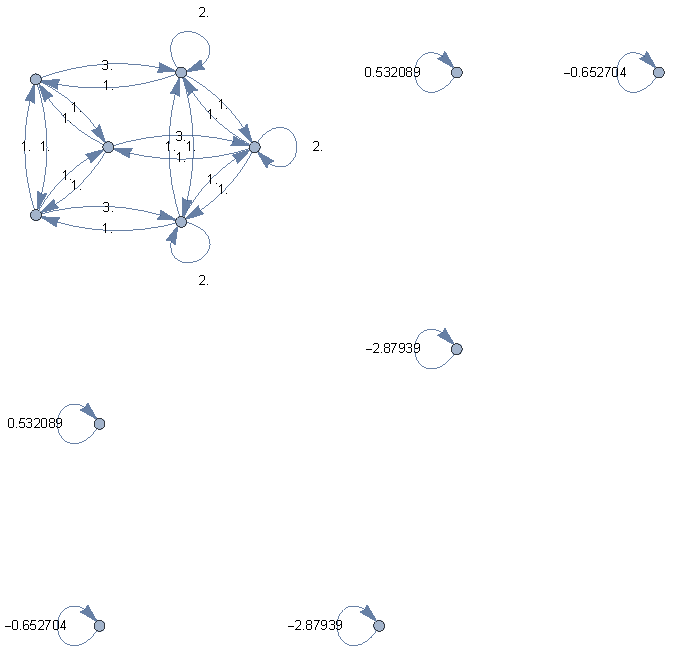
\includegraphics[scale=.8]{ex1_2}\\
\end{center}
where $\lambda_i\in\{-0.652704,-2.87939,0.532089,0.532089,-2.87939,-0.652704\}$ which are 6 eigenvalues of the adjacency matrix. We note here that this matrix does in fact have a automorphism of order 3, which we form in the next step.\\
(c) Now we form our new automorphism to act on the above matrix.
$$\phi_2=(1,2,3)(4,5,6)$$  $\ell_2$=3.  We set $i=2$ and return to step (a)
\\

\emph{Round 2}\\

(a) Now we choose $\cT_f=\{7,8,9,10,11,12\}$ and $\cT_0=\tilde{\cT_0}=\{1,4\}$
\\
(b) We need to reorder the rows and columns of $M(1)$ in order to perform the next decomposition so that transversals are together, i.e. the order of vertices will be $\{7,8,9,10,11,12,1,4,2,5,3,6\}$ as follows:
\[
M(1)'=
\left(\begin{matrix}
\lambda_1&0&0&0&0&0&0&0&0&0&0&0\\
0&\lambda_2&0&0&0&0&0&0&0&0&0&0\\
0&0&\lambda_3&0&0&0&0&0&0&0&0&0\\
0&0&0&\lambda_4&0&0&0&0&0&0&0&0\\
0&0&0&0&\lambda_5&0&0&0&0&0&0&0\\
0&0&0&0&0&\lambda_6&0&0&0&0&0&0\\
0&0&0&0&0&0&2&1&1&0&1&0	\\
0&0&0&0&0&0&3&0&0&1&0&1	\\
0&0&0&0&0&0&1&0&2&1&1&0 \\
0&0&0&0&0&0&0&1&3&0&0&1	\\
0&0&0&0&0&0&1&0&1&0&2&1	\\
0&0&0&0&0&0&0&1&0&1&3&0	\\
\end{matrix}\right)
\]\\
Now we form the new $S$ matrix for this step,
$$S=\left(\begin{matrix}
 I_2 & I_2 \\
\omega I_2&\omega^2 I_2\\
\omega^2 I_2&\omega^4 I_2\\
\end{matrix}\right)$$
where $\omega=e^{2\pi i/3}$. We use this $S$ in the definition of $T$
\[
T = \left[\begin{array}{l | l | l}
I_6 & 0 & 0 \\\hline
0 & I_{2} &  \\
0 & I_{2} & S \\
0 & I_{2} &  \\
\end{array}\right].
\]
Now we can find $M(2)$ and its associated adjacency graph.
\begin{center}
$
M(2)=TM(1)'T^{-1}=
\left(\begin{matrix}
\lambda_1&0&0&0&0&0&0&0&0&0&0&0\\
0&\lambda_2&0&0&0&0&0&0&0&0&0&0\\
0&0&\lambda_3&0&0&0&0&0&0&0&0&0\\
0&0&0&\lambda_4&0&0&0&0&0&0&0&0\\
0&0&0&0&\lambda_5&0&0&0&0&0&0&0\\
0&0&0&0&0&\lambda_6&0&0&0&0&0&0\\
0&0&0&0&0&0&4&1&0&0&0&0	\\
0&0&0&0&0&0&3&2&0&0&0&0	\\
0&0&0&0&0&0&0&0&1&1&0&0 \\
0&0&0&0&0&0&0&0&3&-1&0&0	\\
0&0&0&0&0&0&0&0&0&0&1&1	\\
0&0&0&0&0&0&0&0&0&0&3&-1	\\
\end{matrix}\right).
$
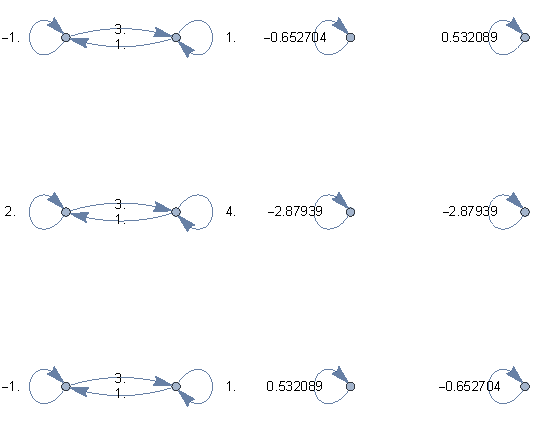
\includegraphics[scale=.8]{ex1_3}
\end{center}
(c) Because $i=2$, the decomposition is complete and there is no need to to find $\phi_2$.
%\afcomm{Here's where we fix the previous example using this new idea}
\end{example}

 \begin{prop}\label{prop:dd}
Let $\phi$ be an automorphism of a graph $G=(V,E,w)$ with automorphism compatible matrix $M$.  Suppose that $\phi$ has order $p^N\ell$, with $p$ a prime which does not divide $\ell$. Then $\psi = \phi^{\ell}$ is an automorphism of $G$ with order $p^N$.  We can construct an automorphism $\tilde{\phi}$ associated with the equitable decomposition of $M$ over $\psi$ of order $\ell$ such that the divisor matrix $(M_\psi)_{\tilde{\phi}} = M_\phi$.
\end{prop}

We will need the following lemma to prove this Proposition.
\begin{lem}\label{lem:compatible}
 Note that for each $k = 1, \ldots N$,  $p^k$ and $\ell$ are relatively prime, therefore there must exist integers $A_k$ and $B_k$ such that
\[
1 = \ell A+ p^N B.
\]
 Following the notation and hypotheses of Theorem \ref{thm:fullprimedecomp}, $\phi^{1-\ell A}$ is an automorphism of each $\tM_k$.
   \end{lem}
 \begin{proof}[Proof of Lemma]
 By hypothesis, $M$ is compatible with $\phi^{1-\ell A}$.  Next, we assume that $\tM_{k-1}$ is as well. Note that $a$ and $\phi^{1-\ell A}(a)$ must both be in $\cT_F$ or neither (for the $k$th stage of the decomposition). Second, notice that if $a \in \cT_m$ (in the $k$th stage of the decomposition), then
 \[
\phi^{1-\ell A}(a) = \phi^{p^NB}(a) = \phi^{p^k(p^{N-k}B)}(a)
 \]
 must also be an element of $\cT_m$. Thus, if we interpret the indices of the rows and columns of $\tM_k$ to be those in $\cT_F \cup \cT_0 \cup \cdots \cT_{p^{k-1}-1}$, then $\phi^{1 - \ell A}$ is a closed map on the indices of $\tM_k$.

 We wish to show that for any $a$, $b$ which are indices appearing in $\tM_k$,
 \begin{equation}\label{eq:compatible}
 \tM_k(\phi^{1-\ell A}(a),\phi^{1-\ell A}(b)) = \tM_k(a,b).\end{equation}

Lemma \ref{lem:Dallas} and  Proposition \ref{prop:primepower} give
\begin{center}
$
 \tM_k(\phi^{1-\ell A}(a), \phi^{1-\ell A}(b)) = \left\{\begin{array}{ll}
 \tM_{k-1}(\phi^{1-\ell A}(a), \phi^{1-\ell A}(b)) & \text{ if } b \in \cT_F \\
 p\tM_{k-1}(\phi^{1-\ell A}(a), \phi^{1-\ell A}(b)) & \text{ if } b \notin \cT_F, \ a \in \cT_F \\
 \sum_{m=0}^{p-1}\tM_{k-1}(\phi^{1-\ell A}(a), \phi^{m\ell p^{k-1}}\phi^{1-\ell A}(b)) & \text{ if } b \in \cT_F, \ a \notin \cT_F  \\
 \end{array}\right.
 $\\[4mm]

$
\hspace*{4cm} =\left\{\begin{array}{ll}
 \tM_{k-1}(\a,b)= \tM_k(a,b) & \text{ if } b \in \cT_F \\
 p\tM_{k-1}(a, b) = \tM_k(a,b) & \text{ if } b \notin \cT_F, \ a \in \cT_F \\
 \sum_{m=0}^{p-1}\tM_{k-1}(a, \phi^{m\ell p^{k-1}}(b)) = \tM_k(a,b)& \text{ if } b \in \cT_F, \ a \notin \cT_F  \\
 \end{array}\right. .
 $
 \end{center}
 All three cases will give the result in Equation \ref{eq:compatible} because, by assumption, $\tM_{k-1}$ is compatible with $\phi$. (In the third case notice that $\phi^{m\ell p^{k-1}}\phi^{1-\ell A}(b) =\phi^{1-\ell A}\circ \phi^{m\ell p^{k-1}}(b)$)
 \end{proof}


\begin{proof}[Proof of Proposition]
Let $M$ be an automorphism compatible matrix of the graph $G$ and $\phi\in Aut(G)$. For ease of notation, let $M(i,j)=M_{ij}$, the $ij^{th}$ element of $M$.

Then, $\psi=\phi^{\ell}$ must have order $p^N$ and thus we can use Theorem \ref{thm:fullprimedecomp} to decompose $M$ with respect to this automorphism.

We follow the procedure outlined in the previous propositions and theorems, but we must choose our transversals more carefully.

%(Recall that at each step we have to choose an element from each orbit of maximal length. )
Let $\so_\phi(a)$ be an orbit of $\phi$  of length $p^km$ for some integer $m$.   Then, $\so_\phi(a) = \so_\psi(a) \cup \cdots \cup \so_{\psi}(\phi ^{m-1} a) $.  For each such orbit we add the elements $\{a, \phi^{p^k}(a), \ldots, \phi^{(m-1)p^k}(a)\}$ to $\cT_0$ for \afcomm{that} step. Since $p^k$ and $\ell$ are relatively prime, no two elements of any power of a transversal can be in the same orbit under $\psi$. We can now define our automorphism $\tilde{\phi}$ by
\[
\tilde{\phi}(a) =%\left\{\begin{array}{ll}
%\phi^p(a) & a \in  \cT_F\cup \cT_0 \\
 \phi^{(1 - \ell A)}(a)  = \phi^{p^k(p^{N-k})B}.%& a  \in \cT_{p^{k-1}}, \ldots, \cT_{p^k-1} \text{ in the } N-k+1th \text{ decomposition}.
% \end{array}\right.
\]



%Clearly this map is well-defined since the size of an orbit is well-defined.
The powers of transversals are made up of unions of sets like $\{a, \phi^{p^k}(a), \ldots, \phi^{(m-1)p^k}(a)\}$, so $\tp$ is closed on each $\cT_m$ (recall that the order of $a$ in this example is $mp^k$, so $\phi^{p^k} ( \phi^{(m-1)p^k}(a)) = a$).

Now we show that this is an automorphism of the decomposed graph.
Let $M_N = \tM_N \oplus \hM_N \oplus \hM_{N-1} \oplus  \cdots \oplus \hM_1$ be the matrix obtained by the $N$th decomposition.
We consider each block matrix $_iB_j$ in $\hM_i$. For $j\neq 0$, and $a$ and $b$ both in $\cT_{p^{k-1}}, \ldots, \cT_{p^k-1} $ for $k = N-i+1$ in the $i$th decomposition.

\[\begin{array}{c}
\displaystyle{
_iB_j(\tilde{\phi}(a),\tilde{\phi}(b)) = \sum_{m=0}^{p^k-1}\omega_{p^k}^{m\gamma_j}\tM_{i-1}(\tilde{\phi}(a), \phi^{\ell m}(\tilde{\phi}(b)) =
\sum_{m=0}^{p^k-1}\omega_{p^k}^{m\gamma_j}\tM_{i-1}(\phi^{(1 - \ell A)}(a), \phi^{\ell m}(\phi^{(1 - \ell A)}(b))
}\\[2mm]
\displaystyle{
=\sum_{m=0}^{p^k-1}\omega_{p^k}^{m\gamma_j}\tM_{i-1}(\phi^{(1 - \ell A)}(a), \phi^{(1 - \ell A)}(\phi^{\ell m}(b))= \sum_{m=0}^{p^i-1}\omega_{p^k}^{m\gamma_j}\tM_{i-1} (a, \phi^m(b)) = \ _iB_j(a,b),
}
\end{array}
\]
by Lemma \ref{lem:compatible}.

Now we must show that  $\tp$ is compatible with $\tM_N $.  We have already shown that $\tM_N = M_{\phi^\ell}$, so we show that $M_{\phi^\ell}(\tp(a), \tp(b)) = M_{\phi^\ell}(a,b)$.

\[\begin{array}{c}
\displaystyle{
M_{\phi^\ell}(\tp(a), \tp(b)) = \sum_{r \in \so_{\phi^\ell}(\tp(b))} M(\tp(a), r) =
\sum_{r \in \so_{\phi^\ell}(\phi^{(1 - \ell A)}(b))} M(\phi^{(1 - \ell A)}(a), r)}\\[10mm]
\displaystyle{
= \sum_{r \in \so_{\phi^\ell}(b)} M(\phi^{(1 - \ell A)}(a), \phi^{(1 - \ell A)}(r)) = \sum_{r \in \so_{\phi^\ell}(b)} M(a, r) = M_{\phi^\ell}(a,b)
}\end{array}
\]


Finally, we need to show that decomposing via $\psi$ and then $\tp$ give the same equitable partition as just using $\phi$ to begin with.
\[
\left(M_{\phi^\ell}(a,b)\right)_{\tp} =  \sum_{r \in \so_{\tp}(b)}  \sum_{s \in \so_{\phi^\ell}(r)} M_{\phi^\ell}(a,s) = \sum_{r \in \so_{\phi}(b))} M(a,r) =\left(M_{\phi}(a,b)\right) .
\]
Since $S = \so_{\phi^\ell}(b) = \{\phi^x(b) \ | \ x \cong 0 \mod \ell\},$ and
\[
\tp^tS = \{\phi^t(b') \ | \ b' \in S\} = \{\phi^x(b) \ | \ x \cong t \mod \ell\}.
\]


%
%Next, we assume that $p$ appears only once in the prime decomposition of $\ell$, that is, $(p,k) = 1$.  In order to perform an equitable decomposition with respect to $\psi$, we choose a semi-transversal in the following way: For each orbit of $\phi$ that is not fixed by $\psi$, pick one element an element $a$.  Then we add the elements of the set $
% \{ a, \phi^{p}(a), \phi^{2p}(a), \ldots, \phi^{(k-1)p}(a) \}.
%$ to $\cT_0$.
%
%To see that this is a semi-transversal, notice that the element $a$ gives $k$ orbits under $\psi$ and there are $k$ elements in the set listed above.  Next we show that the elements in the above set must come from different orbits.  Suppose that $\phi^{qp}$ and $\phi^{q'p}$ are in the same orbit under $\psi$, then
%$\phi^{qp} =\psi^s  \phi^{q'p} = \phi^{ks + q'p}$. Thus, $k \ | \ (q - q')$, a contradiction.
%
%We let $\mathcal{U}$ denote the set of vertices fixed by $\psi$. Now for each semi-transversal we define a map $\phi_m:\cT_m \to \cT_m$ with $\phi_m(i)$ given by $\phi_0(i) = \phi^{p}(a)$, and $\phi_m = \psi^m \phi_0 \psi^{-m}$.
%We can now define $\tilde{\phi}: V(\tilde{G}) \to V(\tilde{G})$ by $\tilde\phi \equiv \phi_{\alpha}\phi_1\phi_2\cdots\phi_{k-1}$. Since each $\phi_m$ acts only on  $\mathcal{T}_m$,  we need only demonstrate that each $\phi_m$ is an automorphism on $B_m$ (see Theorem \ref{thm:2}) in order to show that $\tilde{\phi}$ acts trivially on the vertices in $\cU$.  Let $a,b\in \mathcal{T}_m$.
%Recall from \ref{??} that
%\afcomm{\[
%B_m = \sum_{j=0}^{k-1} \omega^{mj} M[\cT_0,\cT_j],
%\]}
%Thus, if $b, b' \in \cT_m$, and we wish to calculate the $(b,b')$ entry in $B_m$, we must examine the corresponding entries in $M$ which come from $\cT_0$ and $\cT_j$. This is demonstrated in the first equality below:
%
%\begin{align*}
%B_m(\phi_m(b),\phi_m(b'))&=\sum_{j=0}^{k-1}\omega^{mj}
%M(\psi^{-m}\phi_m(b), \psi^{j-m}\phi_m(b'))
%=\sum_{j=0}^{k-1}\omega^{mj} M(\phi_0\psi^{-m}(b), \psi^{j}\phi_0\psi^{-m}(b'))\cr
%&=\sum_{j=0}^{k-1}\omega^{mj} M(\phi^{p}\psi^{-m}(b), \phi^{p}\psi^{j-m}(b'))
%=\sum_{j=0}^{k-1}\omega^{mj} M(\psi^{-m}(b), \psi^{j-m}(b'))= B_m(b,b')
%\end{align*}
%where the third equality holds because $\psi = \phi^k$, and the fourth equality is the defining property of automorphism compatible matrices. Thus, each $\phi_m$ is an automorphism on $B_m$ and subsequently, $\tilde{\phi} $ is an automorphism on $B$, the decomposition of $M$.
%
%When considering just the divisor matrix, $M_{\phi}$, we find
%$$\begin{array}{l}
%\ds{M_\phi (a,b)=\sum_{s\in \so_\phi(b)}M(a,s)=\sum_{m\in \so_{\tilde{\phi}}(b)}\left( \sum_{s\in\so_\psi(m)}M(a,s)\right)} \ds{ \ =\sum_{s\in\so_{\tilde{\phi}}(b)} M_{\psi}(a,s)=(M_{\psi})_{\tilde{\phi}}(a,b)}
%\end{array}$$
%The second equality holds because $$\so_\phi(s)=\bigcup_{t\in\so_{\tilde{\phi}}(S)} \so_\psi(t)$$ %the set of all elements $s$ in the orbits under $\psi$ of all $\phi^m(j) $ for $0\leq m \leq k-1$, are the same as the set of all elements in the orbit under $\phi$ of $j$.
%Hence, $M_{\phi}=(M_{\psi})_{\tilde{\phi}}$.
%
%% The last equality follows from observing if $\so_\psi(j)$ is the orbit of $j$ under $\psi$, then the union of
\end{proof}
\noindent \dscomm{ Perhaps here we add the ULTIMATE THEOREM, which essentially says using the previous Proposition we can completely Equitably Decompose over ANY automorphism...}
\\

We now give an algorithm for completely decomposing a graph with respect to any of its automorphisms.

\marginpar{\dscomm{This is the Algorithm I have come up with...}}

\begin{center}
\emph{Performing Equitable Decompositions of General Type}
\end{center}

\begingroup\raggedright\leftskip=20pt\rightskip=20pt

For a graph $G$ with automorphism compatible matrix $M$ and nonuniform automorphism $\phi$ of order $\ell $ with prime factorization ${\ell=p_0^{N_0}p_1^{N_1} \cdots p_{h-1}^{N_{h-1}}}$, set $M(0)  = M$, $\ell_0 = \ell$, and $\phi_0 = \phi$.  We perform $h$ sequential decompositions of $M$, one for each prime in our factorization. To begin we start with $i = 0$, and move to \emph{Step a.}\m

\vspace{0.1in}

%\noindent \textbf{Remark.} For the first decomposition we start with only $G_0$ and $\phi_0$.  For all the other decompositions we start Step a with a graph $G_i = G_{i-1}^0 \cup \ldots \cup G_{i-1}^{r_i-1}$, and an automorphism of $G_i$, $\phi_i = \phi_{i-1,0}\cdots\phi_{i-1,r_{i-1}}$ where for all $a \in \{0, \ldots, r_{i-1}\}$, $\phi_{i-1,a}$ is an automorphism of $G_{i-1}^a$ with order dividing $\ell_i$  (so, for ease of notation let $G_{-1}^1 = G$ and $\phi_{-1,1} = \phi$). \textcolor{red}{should this be $G_{-1}^0 = G$ and $\phi_{-1,0} = \phi$?}\\

\noindent\emph{\textbf{Step a:}} \emph{Let $\ell_{i+1} = \ell_i/p_i^{N_i}$.  Form the automorphism $\psi_{i} = \phi_i^{\ell_{i+1}}$}, which has order $p_i^{N_i}$.\\
%Notice that if we also let $\psi_{i,a}= \phi_{i-1,a}^{\ell_{i+1}}$, then $\psi_{i,a}$ is a basic (or trivial) automorphism on $G_{i-1}^a$. \s
\noindent\emph{\textbf{Step b:}} \emph{Perform the $N_i$ equitable decompositions of $M(i)$ using the above algorithm for decomposing a matrix over an automorphism $\psi_i$ order $p_i^{N_i}$. Throughout this process we chose a semi-transversal as prescribed in proof of Proposition \ref{prop:dd}, meaning, on the $k^{th}$ step we need to define a semi-transversal $\cT_0$ with elements chosen from orbits of $\phi_i$.  We are free to choose one element $a$ for each orbit of $\phi_i$ of length $mp_i^{N_i-k}$, but then we must also include $\{ \phi_i^{p_i^{N_i-k+1}}(a),\dots,\phi_i^{(m-1)p_i^{N_i-k+1}(a)}\}$ to get a semi-transversal of the orbits of $\psi_i$.  Finally we define $M(i+1)$ to be the resulting matrix of the above algorithm.}

%We can think of this as a decomposition using the automorphism $\psi_{i}$ on the graph $G_i$ with transversal $\mathcal{T}^i$, or as simultaneously decomposing the graphs $G_{i-1}^a$ using the automorphisms $\psi_{i,a}$ with transversals $\mathcal{T}^{i,a}$.  The former makes for much nicer notation, while the latter gives a better description of the final decomposition. \s\s

\noindent\emph{\textbf{Step c:}} \emph{Define $\phi_{i+1}=\tilde{\phi}_i=\phi_i^{1-\ell_i A}$, where $A$ is the integer chosen so that $1=\ell_{i+1} A+p_i^{N_i}B$ as described in the proof of Proposition \ref{prop:dd}.
%, where $(\phi_i)_j$ is $\phi$ with every element $a$ in its cycle decomposition replaced as:  $a\mapsto \mathcal{T}_j \cap \so_{\psi_i}(a)$. %\noindent\emph{\textbf{Step c:}} \emph{Use Proposition \ref{prop:relabel} to define  $G_{i+1} = G_i^0\cup \cdots \cup G_i^{r_i}$ and to construct a new automorphism $\phi_{i+1}$ on $G_{i+1}$.}\\
%If we use Proposition \ref{prop:relabel} on the graphs $G_{i-1}^a$ with automorphism $\phi_{i-1,a}$ and prime $p_i$, {then each graph $G_{i-1,a}$ where $\psi_{i,a}$ is non-trivial is} decomposed into $p_i$ disjoint graphs:
%\[
%(G_{i-1,a})_0 , (G_{i-1,a})_{2}, \ldots, (G_{i-1,a})_{p_i-1},
%\]
%{with the new} automorphisms $\phi_{i,a,1}, \ldots, \phi_{i,a,p_i}$ (Notice that $(G_{i-1,a})_0= (G_{i-1,a})_{\psi_{i,a}}$).  We relabel these graphs and automorphisms, $G_{i,0}, \ldots, G_{i,r_i}$ and $\phi_{i,0}, \ldots, \phi_{i,r_i}$, {respectively}.
If $i < h$, then set $i = i+1$ and return to \emph{Step a}.  Otherwise, the decomposition is complete.}

%Upon the completion of the decomposition, we will have $r_h$ distinct graphs %$G_{h}^a$
%with $n_a$ vertices, where $1 \leq n_a \leq r$, $r$ is the number of distinct cycles (including any trivial cycles) in $\phi$, and $\sum n_a = n$. Notice that in the last round, it is not necessary to find $\phi_h$.

\par\endgroup

\vspace{0.1in}

\noindent The procedure described in Steps $a$--$c$ allows one to sequentially decompose a matrix $M$ over any of its automorphisms. By extension we refer to the resulting matrix as an \emph{equitable decomposition} of $M$ over $\phi$. The following example illustrates an equitable decomposition over an automorphism that is neither basic nor separable.

\begin{example}\label{ex:18}
Consider the following graph and associated adjacency matrix $M$.\\
\begin{center}
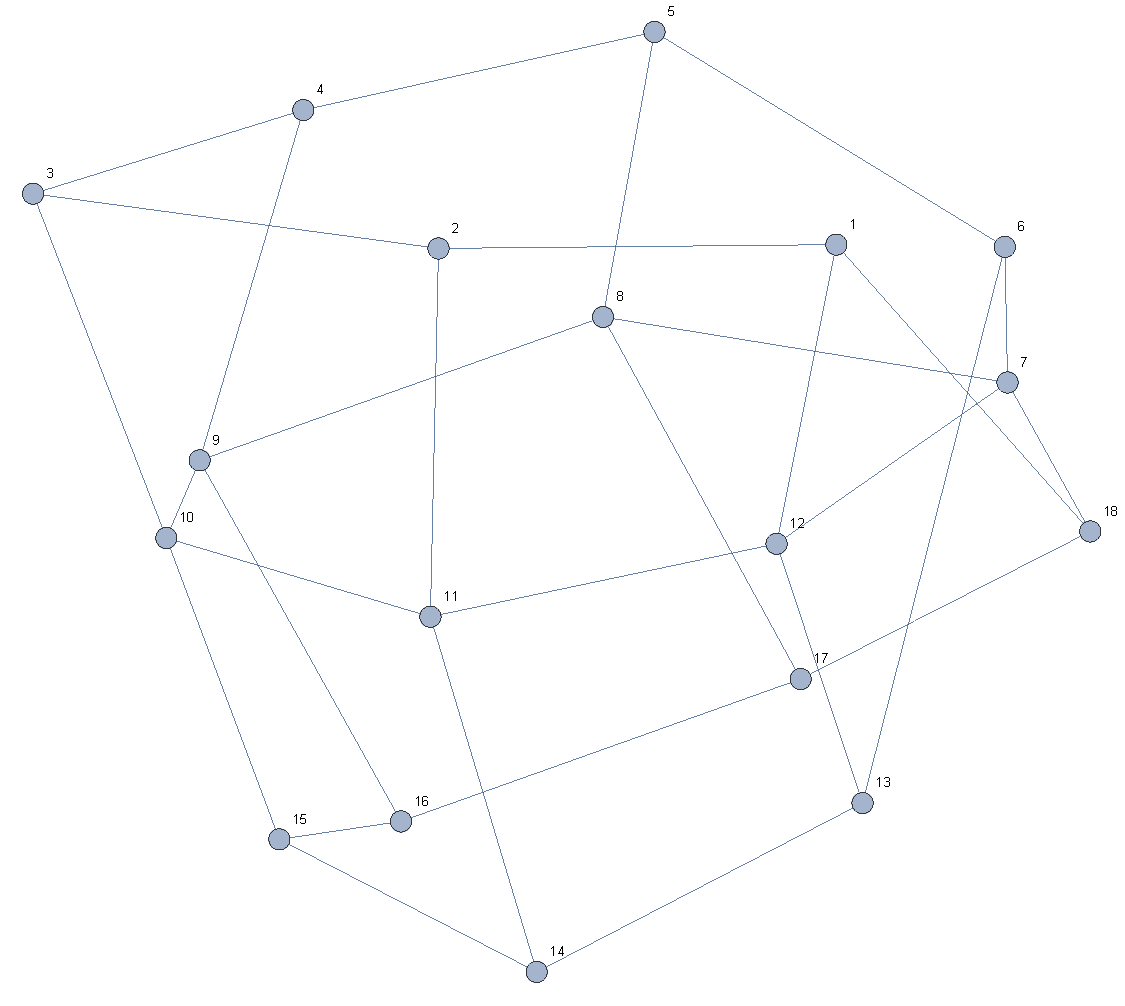
\includegraphics[scale=.5]{ex2_0.pdf}
\end{center}
% \[
% M=
% \left(\begin{matrix}
% 0&1&0&1&1&1&1&1&0\\
% 1&0&1&0&1&1&1&0&1\\
% 0&1&0&1&1&1&1&1&0\\
% 1&0&1&0&1&1&1&0&1\\
% 1&1&1&1&0&1&1&0&0\\
% 1&1&1&1&1&0&1&0&0\\
% 1&1&1&1&1&1&0&0&0\\
% 1&0&1&0&0&0&0&0&0\\
% 0&1&0&1&0&0&0&0&0\\
% \end{matrix}\right)
% \]
This graph has the automorphism $(1,2,3,4,5,6,7,8,9,10,11,12)(13,14,15,16,17,18)$, which has order $12= 4^2 \cdot 3$thus $p_0=2,N_0=2$ and $p_1=3,N_1=1$.  Because there are 2 distinct prime factors we will go through the steps (a)-(c) 2 times. We start with $i=0$, $M(0)=M$, $\ell_0=12$, $\phi_0=\phi$.\\
\noindent Round 1\\
\emph{step (a)}:  We start with $\ell_1=\ell_0/p_0^{N_0}=12/2^2=3$ and thus $$\psi_0=\phi_0^3=(1,4,7,10)(2,5,8,11)(3,6,9,12)(13,16)(14,17)(15,18)$$.\\
\emph{step (b)}: Now we run though algorithm for decomposing a graph order $p^N$ (first algorithm in this paper) on M(0) using the automorphism $\psi_0=\psi_{0,0}$ (the second subscript keeps track automorphism within the sub-algorithm). This will require 2 iterations of the sub-algorithm since $N_0=2$.  In the first round of this sub-algorithm, we have three orbits whose length is equal to 4.  When choosing our semi-transversal $\tau_0$, we a free to choose any element from the first orbit, but based on that choice the other two elements of $\cT_0$ are given to us by the algorithm.  We freely choose $1\in \tau_0$.  Therefore $\cT_0=\{1,\phi_0^4(1),\phi_0^{2\cdot 4}(1)\}=\{1,5,9\}$. It follows that $\cT_1=\phi(\tau_0)=\{4,8,12\}$, $\cT_2=\phi^2(\tau_0)=\{7,11,3\}$, and $\cT_3=\phi^3(\tau_0)=\{10,2,6\}$. The remaining vertices are put into $\cT_f=\{13,14,15,16,17,18\}$ since they are contained in orbits of $\psi_{0,0}$ whose order is less than $p_0^{N_0}=4$.  The first round this algorithm will result in a decomposed matrix $M(0)(1)$ whose adjacency graph has the following form
\begin{center}
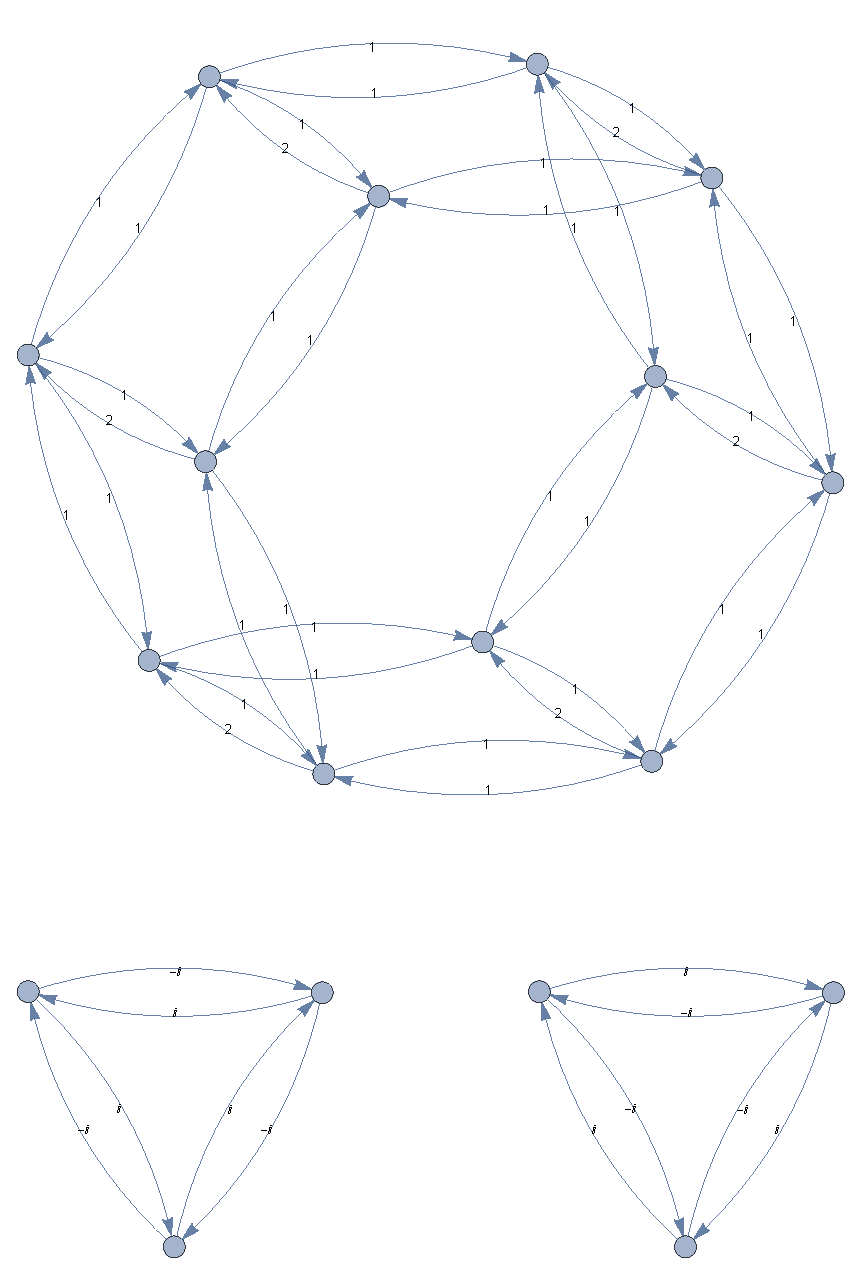
\includegraphics[scale=.5]{ex2_1.pdf}
\end{center}
% \[
% M(0)(1)=\left(\begin{matrix}
% \end{matrix}\right)
% \]
In the second iteration of the sub-algorithm, we use \eqref{eq:6} to find the new automorphism $$\psi_{0,1}=(1,4)(5,8)(9,12)(13,16)(14,17)(15,18)$$ thus we have 6 cycles of length $2$. We now must choose the semi-transversals for the next step. We begin with all the elementfrom $\cT_0$ in the previous set $\{1,5,9\}$. To have it transverse all the orbits, we also need to add some vertices. We are free to choose any element from the remaining orbits of $\psi_{0,1}$, so we choose $13\in\cT_0$, and then we also add $\{\phi ^{2}_0(13),\phi ^{2\cdot 2}_0(13)\}=\{15,17\}$.  Putting these together gives our new $\cT_0=\{1,5,9,13,15,17\}$, and also $\cT_1={4,8,12,16,18,14}$.  Using these transversals, the second iteration of the sub-algorithm results in an adjacency matrix $M(0)(2)=M(1)$ which the corresponding weighted adjacency graph

\begin{center}
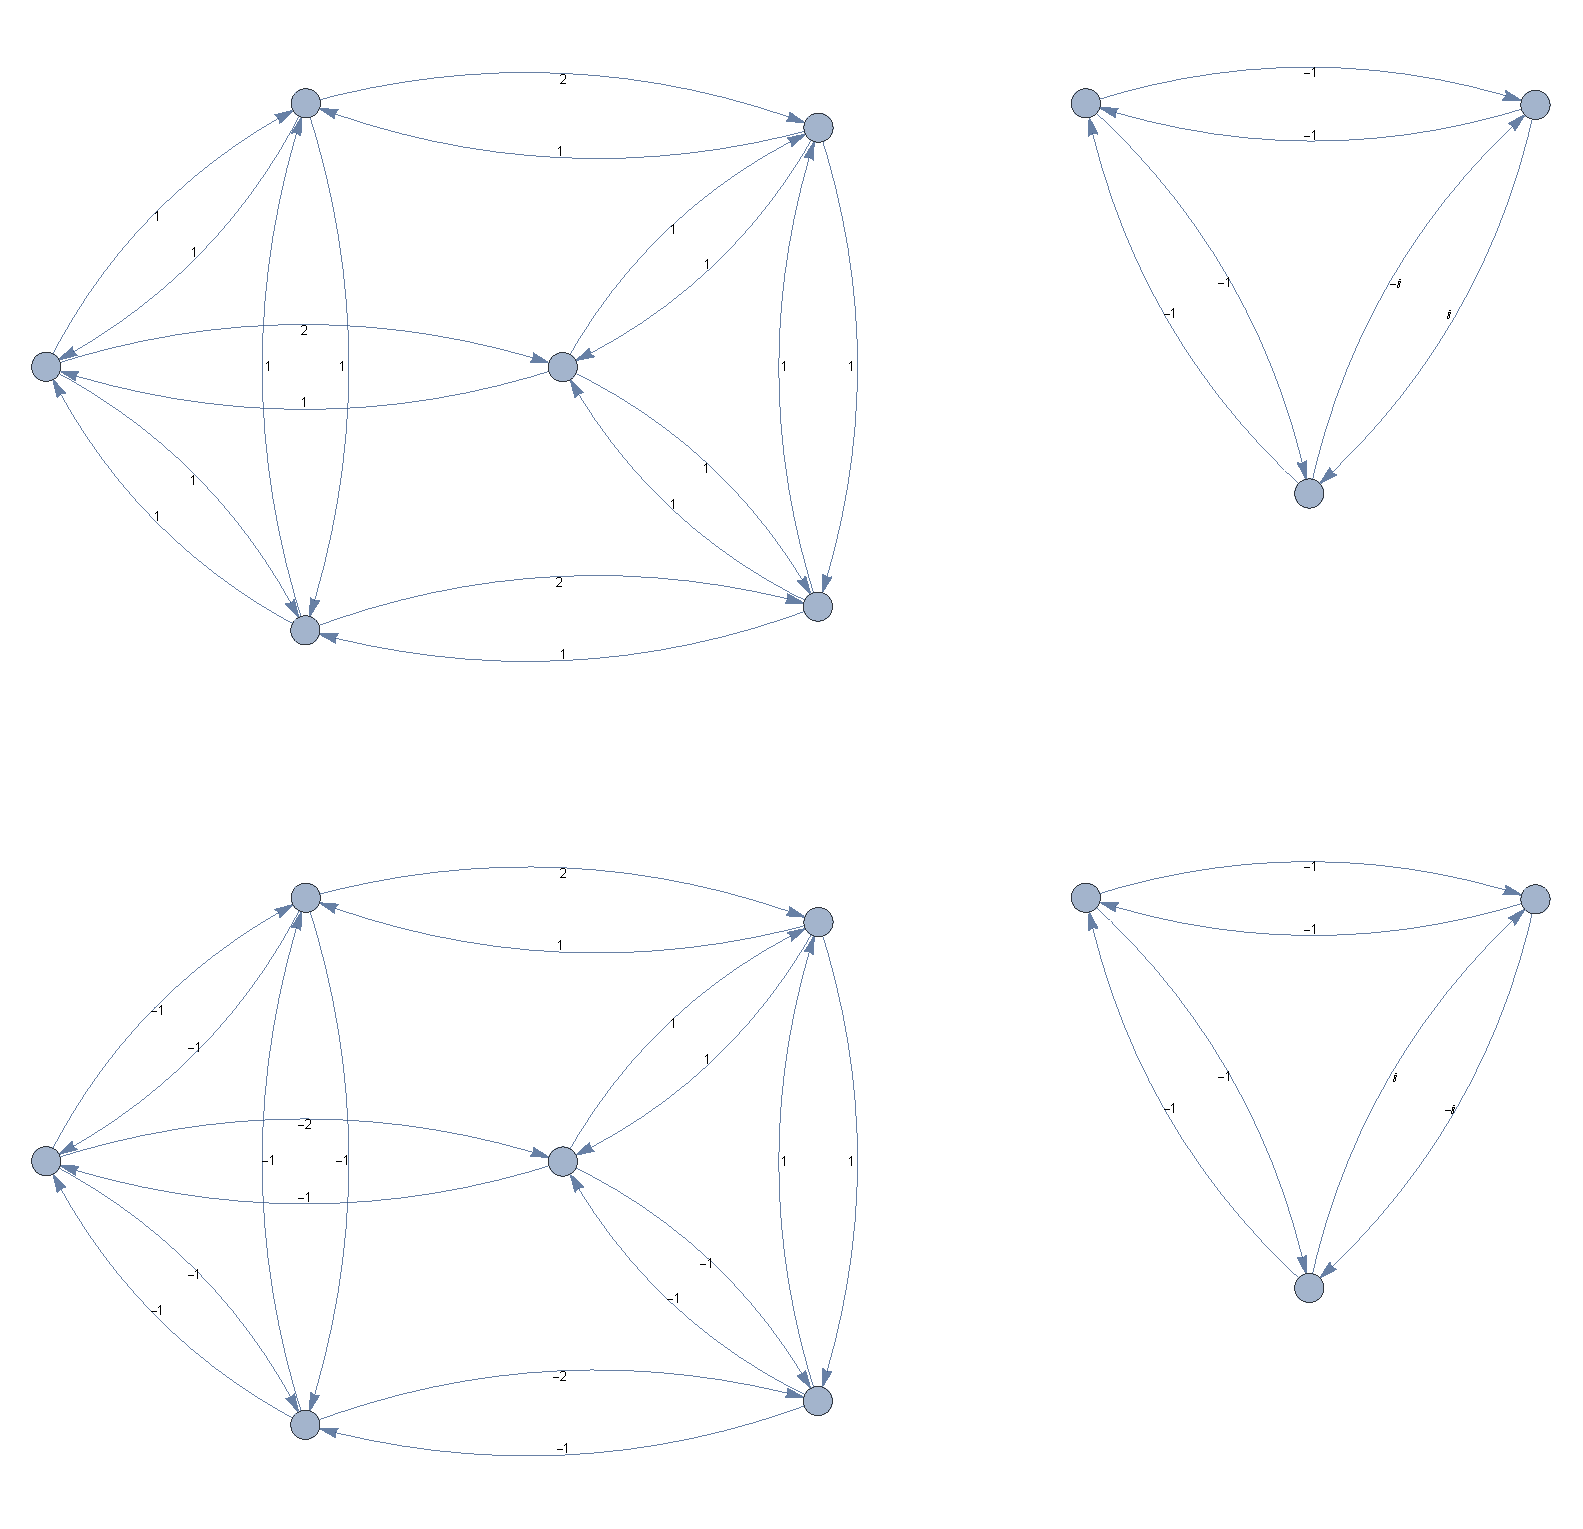
\includegraphics[scale=.3]{ex2_2.pdf}
\end{center}

%after matrix reordering $\{3,8,2,9,5,6,7,1,2\}$:
% \[
% M(1)=M(0)(2)=\left(\begin{matrix}
% -2&	1&	0&	0&	0&	0&	0&	0&	0&\\
% 2&	0&	0&	0&	0&	0&	0&	0&	0&\\
% 0&	0&	2&	1&	1&	1&	1&	0&	0&\\
% 0&	0&	2&	0&	0&	0&	0&	0&	0&\\
% 0&	0&	4&	0&	0&	1&	1&	0&	0&\\
% 0&	0&	4&	0&	1&	0&	1&	0&	0&\\
% 0&	0&	4&	0&	1&	1&	0&	0&	0&\\
% 0&	0&	0&	0&	0&	0&	0&	0&	0&\\
% 0&	0&	0&	0&	0&	0&	0&	0&	0&\\
% \end{matrix}\right)
% \]

\emph{step (c)}: Now with our new matrix, we need to determine the automorphism for the next step.
$\phi_{1}=\phi_0^{(1-A\ell_{1})}$, where $A=-1$, since $1=(-1)\ell_{1}+(1)p_0^{N_0}=(-1)3+(1)4$.  Thus \begin{align*}
\phi_{1}=\phi_0^{(1-(-1)3)}=\phi_0^4=[(1,2,3,4,5,6,7,8,9,10,11,12)(13,14,15,16,17,18)]^4\\
=(1,5,9)(2,6,10)(3,7,11)(4,8,12)(13,17,15)(14,18,16)
\end{align*}
\\
Round 2\\
\emph{Step a}: Now $\ell_2=1$, thus $\psi_1=\phi_1^1$\\

\noindent \emph{Step b}: On this step we only need to run through the above algorithm once since the order of our automorphism is $3^1$.  During this step we do not need to be worried about how we choose the transversal for the decomposition because this is the final step and the transversal only need to be carefully chosen to guarantee that the resulting decomposed graph contains a symmetry for the next round. Thus after running through the algorithm 1 on $M(1)$ and with automorphism $\psi_1$ we get $M(2)$ with the following adjacency graph.

\begin{center}
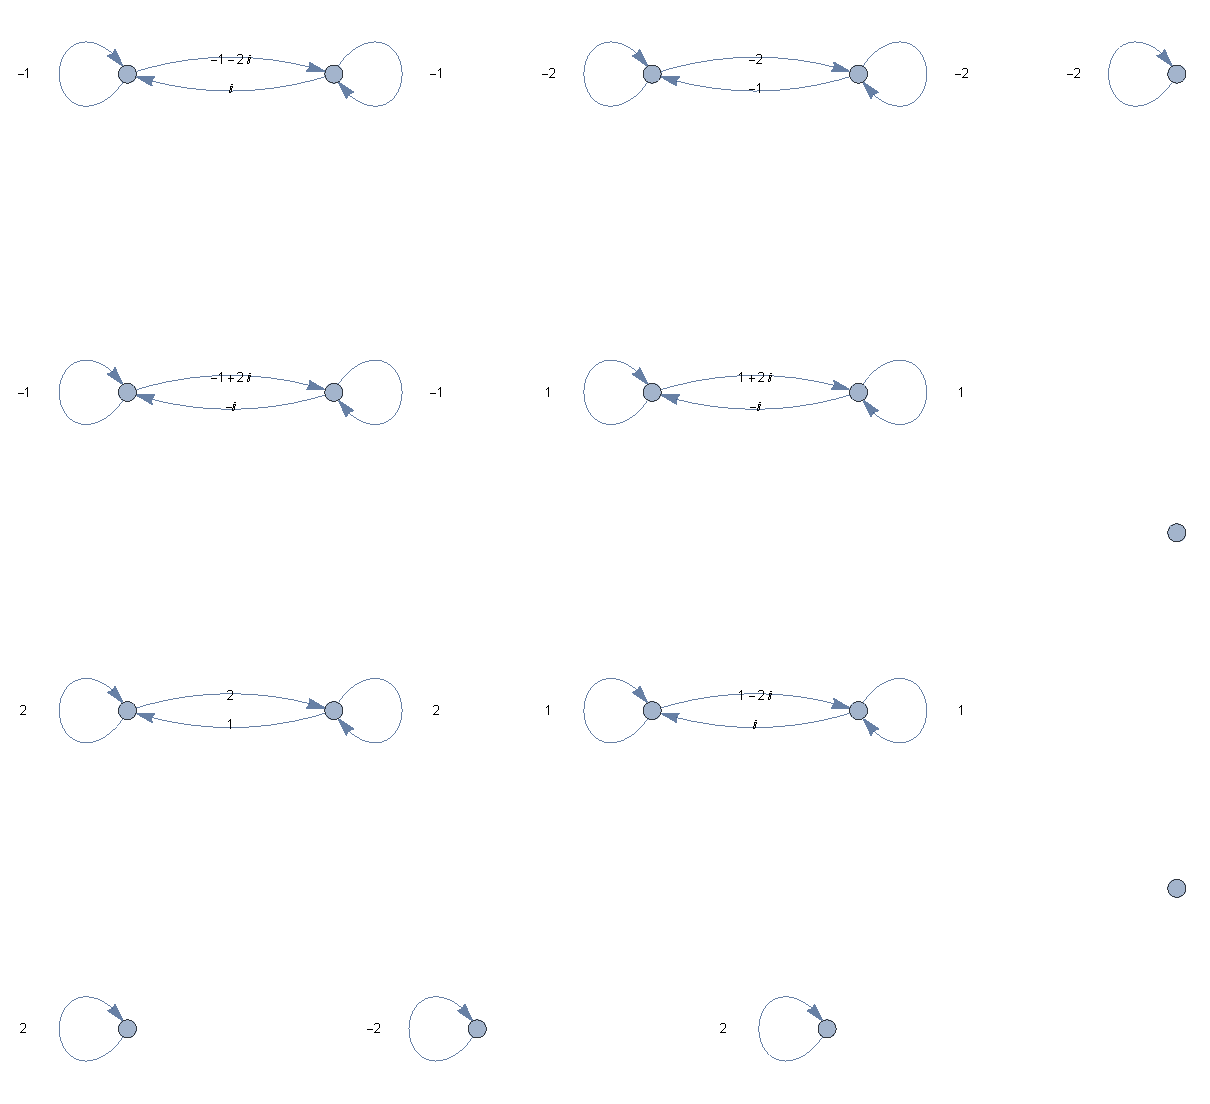
\includegraphics[scale=.5]{ex2_3.pdf}
\end{center}
% After reorder the matrix again, we get
% \[
% M(2)=M(1)(1)=\left(\begin{matrix}
%  0& 0& 0& 0& 0& 0& 0& 0& 0 \\
%   0& 0& 0& 0& 0& 0& 0& 0& 0 \\
%   0& 0& -2& 1& 0& 0& 0& 0& 0 \\
%   0& 0& 2& 0& 0& 0& 0& 0& 0 \\
%   0& 0& 0& 0& -1& 0& 0& 0& 0 \\
%   0& 0& 0& 0& 0& -1& 0& 0& 0 \\
%   0& 0& 0& 0& 0& 0& 2& 4& 0 \\
%   0& 0& 0& 0& 0& 0& 3& 2& 1 \\
%   0& 0& 0& 0& 0& 0& 0& 2& 0 \\
% \end{matrix}\right)
% \]

\emph{Step c}: There is no need to find $\phi_2$ since we cannot decompose this matrix any further.

\end{example}
\section{Extensions and Applications}
As in [paper 2], we describe the form of the eigenvectors for a matrix $M$ given the eigenvectors of the smaller $B_i$ matrices which are a result of the decomposition over an automorphism of size $p^N$.  We can explicitly write down a form for the eigenvectors for a single step in the decomposition.  Starting with the eigenvectors of the final blocks, we can work backwards, each time find the eigenvectors of the previous matrix in the sequence of decompositions.
For a single step we have eigenvectors with essentially the same form that we had in [paper 2].

\begin{theorem}
Let $M$ be an $n\times n$ automorphism compatible matrix of the graph $G$. For $\phi$ an automorphism of $G$ with order $p^N$ and let $\tilde{M} \oplus B_1\oplus \cdots \oplus B_{p^N-p^{N-1}}$ be a single decomposition of $M$ as described in Proposition???. Suppose $\{\mathbf{u}_{m,\ell}:1\leq \ell \leq r\}$ \textcolor{red}{($n=f+rp^N$)}  is a (generalized) eigenbasis for $B_m$  for $1\leq m\leq p^N-p^{N-1}$ and $\{{{\mathbf{u}}_{0,i}}:1\leq i\leq f+rp^{N-1}\}$ is a (generalized) eigenbasis for $\tilde{M}$ and where each ${\mathbf{u}}_{0,i}= {{\mathbf{w}}_i} \oplus {{\mathbf{v}}_i}$ with ${{\mathbf{w}}_i}\in\mathbb{C}^f\text{ and }{{\mathbf{v}}_i}\in\mathbb{C}^{rp^{N-1}}$. Then a (generalized) eigenbasis of $M$ is the set
\begin{equation}\label{eq:vect}
\left\{{{\bf{0}}_f}\, \oplus {\left[ {\mathop  \bigoplus \limits_{j = 0}^{p^N-1} {\omega ^{j \gamma_m}}{{\bf{u}}_{m,\ell}}} \right] ,{{\bf{w}}_i}\,\oplus \left[   {\mathop  \bigoplus \limits_{j = 0}^{p - 1} {{\bf{v}}_i}} \right]\,:1 \leq m \leq p^N-p^{N-1}, 1 \leq \ell \leq r,1 \leq i \leq f + rp^{N-1},\omega=e^{2\pi i/k}\,} \right\}.
\end{equation}

Moreover, if $\mathbf{x}_{m,l}={{\bf{0}}_f}\oplus \left[ {\mathop  \bigoplus \limits_{j = 0}^{p^N - 1} {\omega ^{j\gamma_m}}{{\bf{u}}_{m,l}}} \right]$ and ${{\bf{x}}_{0,i}} =  {{\bf{w}}_i} \oplus \left[{\mathop  \bigoplus \limits_{j = 0}^{p - 1} {{\bf{v}}_i}} \right]$ then the following hold.\\
(i) If $\lambda_{m,\ell}$ is the $\ell^{th}$ eigenvalue of $B_m$ then $\lambda_{m,\ell}\in\sigma(M)$ corresponds to the (generalized) eigenvector $\mathbf{x}_{m,l}$.\\
(ii) If $\lambda_{0,i}$ is an eigenvalue of $M_\phi$ then $\lambda_{0,i}\in\sigma(M)$ corresponds to the (generalized) eigenvector ${{\bf{x}}_{0,i}}$.
\end{theorem}
The proof of the above theorem exactly follows the proof of Theorem 4.1 in \ref{}[paper 2], essentially showing that if $\mathbf{v}$ is an eigenvector of $T^{-1}MT$, then $T\mathbf{v}$ is an eigenvector of $M$. Thus this form described for eigenvectors in the above theorem comes straight from doing this computation.

\begin{example}
Consider the first decomposition performed example \ref{}, we found that $$M(0)(1)=\tilde{M}\oplus B_1\oplus B_2\text{ where } \tilde{M}=\left[\begin{matrix}
F & 2H \\
H^T & B_0 \end{matrix}\right]$$ with$$F=\left[
\begin{matrix}
0 & 1 & 0 & 0 & 0 & 1\\
1 & 0 & 1 & 0 & 0 & 0\\
0 & 1 & 0 & 1 & 0 & 0\\
0 & 0 & 1 & 0 & 1 & 0\\
0 & 0 & 0 & 1 & 0 & 1\\
1 & 1 & 0 & 0 & 1 & 0\\
\end{matrix}\right] \text{, }H=\left[\begin{matrix}
0 & 1 & 0 & 0 & 0 & 0\\
0 & 0 & 0 & 0 & 0 & 1\\
0 & 0 & 0 & 1 & 0 & 0\\
0 & 0 & 0 & 0 & 1 & 0\\
0 & 0 & 1 & 0 & 0 & 0\\
1 & 0 & 0 & 0 & 0 & 0\\
\end{matrix}\right] \text{, }B_0=\left[\begin{matrix}
0 & 0 & 0 & 0 & 1 & 1\\
0 & 0 & 0 & 1 & 0 & 1\\
0 & 0 & 0 & 1 & 1 & 0\\
0 & 1 & 1 & 0 & 0 & 0\\
1 & 0 & 1 & 0 & 0 & 0\\
1 & 1 & 0 & 0 & 0 & 0\end{matrix}\right]$$ and $$
B_1=-B_2=\left[\begin{matrix} 0 & -i & i \\ i& 0 & -i \\ -i &i & 0 \end{matrix}\right]\\
\text{ and }$$

After finding the eigenvectors of $\tilde{M},\ B_1$ and $B_2$ we can immediately write down eigenvectors for the original matrix $M$. For example $$\mathbf{u}_{0,1}=(2,\ -2,\ 2,\ -2,\ 2,\ -2,\ \sqrt{2},\ \sqrt{2},\ \sqrt{2},\ -\sqrt{2},\ -\sqrt{2},\ -\sqrt{2})^T $$ is an eigenvector of $\left[\begin{matrix}
F & 2H \\
H^T & B_0 \end{matrix}\right]$, so $$\mathbf{w_1}=(2, -2,\ 2, -2,\ 2, -2)^T$$ $$\mathbf{v_1}=(\sqrt{2},\ \sqrt{2},\ \sqrt{2}, -\sqrt{2}, -\sqrt{2}, -\sqrt{2})^T.$$  Thus $M$ must have an eigenvector of the form
\begin{multline*}\mathbf{x}_{0,1}=\mathbf{w}_1\oplus\mathbf{v}_1\oplus\mathbf{v}_1\\
=(2, -2,\ 2, -2,\ 2,\ -2, \sqrt{2}, \sqrt{2}, \sqrt{2}, -\sqrt{2}, -\sqrt{2}, -\sqrt{2},\sqrt{2}, \sqrt{2}, \sqrt{2}, -\sqrt{2}, -\sqrt{2}, -\sqrt{2})^T.\end{multline*}  We can also find 11 other eigenvector in this way using the other 11 eigenvectors of $\tilde{M}$. In addition, $\mathbf{u}_{1,1}=(1,\ 1,\ 1)^T$ is an eigenvector of  $B_1$, then another eigenvector of $M$ is \begin{align*}
\mathbf{x}_{1,1}=&\mathbf{0}_6\oplus\mathbf{u}_{1,1}\oplus\omega\mathbf{u}_{1,1}\oplus\omega^2\mathbf{u}_{1,1}\oplus\omega^3\mathbf{u}_{1,1}\\
=&(0,\ 0,\ 0,\ 0,\ 0,\ 0,\ 1,\ 1,\ 1,\ i,\ i,\ i,\ -1,\ -1,\ -1,\ -i,\ -i,\ -i)
\end{align*}.  We can find 5 more eigenvector with this form using the other two eigenvectors of $B_1$ and the three eigenvectors of $B_2$. Thus we can find the complete set of eigenvectors which form the eigenbasis for $M$.

We also note here that had we started with the next step we could have used the eigenvectors of the components of $M(0)(2)$ to to come up with the eigenvectors of $M(0)(1)$ which we used in this example to find the eigenvectors of $M$, and so on.
\end{example}

Another result that can be generalized from \ref{} [paper 2], is that the spectral radius of a nonnegative matrix $M$ is the same as the spectral radius of the divisor matrix $M_\phi$ for any automorphism $\phi$.  A weaker version of this proposition was was proved for the case of $\phi$ a basic or separable automorphism in Proposition 4.3 of \ref{}[paper 2].

\begin{prop}\label{lem:3}\textbf{(Spectral Radius of Equitable Partitions)}
Let $\phi$ be any automorphism of a graph $G$ with $M$ an automorphism compatible matrix. If $M$ is nonnegative and irreducible, then its spectral radius, $\rho(M)$, is the largest eigenvalue of $M_{\phi}$.
\end{prop}

\begin{proof}
  If we can prove that the result holds using the decomposition techniques demonstrated in Lemma \ref{lem:Dallas}, the first step of the case where $\phi$ has order $p^N$, then the general results.  This is because completely decomposing a matrix over a more complex automorphism is done in a sequence of decompositions and if we show the divisor matrix and the end of each step has the desired properties, then induction proves our result.

Thus we assume that $M$ is an irreducible, nonnegative matrix with automorphism $\phi$, where the order of $\phi$ is $p^N$.  We know there is a permutation from \ref{} which will put $M$ into ``double block circulant form" given in Lemma \ref{lem:Dallas}. Using the same notation as in this Lemma, let $\tilde{M}=\left[\begin{array}{rr} F & kH \\ L & B_0 \end{array}\right]$. we need to show that $\rho(\tilde{M})=\rho(M)$.
Lemma \ref{lem:Dallas } describe a matrix $T$ so that \[
T^{-1} M T = \tilde{M}
\oplus B_1 \oplus B_2 \oplus \cdots \oplus B_{p^N-p^{N-1}},
\].
We first claim that $\rho(\tilde{M})\geq\rho(B_j)$ for $1\leq j\leq p^{N}-p^{N-1}.$

To verify this claim, we first need Corollary 8.1.20 in \cite{Horn85} which states that if $N$ is a principal submatrix of $M$ then $\rho(N)\leq\rho(M)$ if $M$ is nonnegative. We see that $B_0$ is a principal submatrix of $\tilde{M}$.  Since $M$ is nonnegative, and $B_0=\sum_{m=0}^{p-1}D_m$, we know $\tilde{M}$ is nonnegative, and  we can conclude that $\rho(B_0)\leq\rho(\tilde{M})$.

Next we must show that $\rho(B_j)\leq\rho(B_0)$ for $1\leq j \leq p^N-p^{N-1}$. For a matrix $P\in\mathbb{C}^{n\times n}$, let $|P|\in\mathbb{R}_{\geq 0}^{n\times n}$ denote the matrix with entries $|P|_{ij}=|P_{ij}|$, i.e. $|P|$ is the entrywise absolute value of $P$. Moreover, if $P,Q\in\mathbb{R}^{n\times n}$ let $P\leq Q$ if $P_{ij}\leq Q_{ij}$ for all $1\leq i,j\leq n$. Theorem 8.1.18 in \cite{Horn85}, states that if $|P|\leq Q$  then $\rho(P)\leq\rho(Q)$. Because
$$\left| {{B_j}} \right| = \left| {\sum\limits_{m = 0}^{p^N - 1} {{{\left( {{\omega ^{m\gamma_j}}} \right)}}{C_m}} } \right| \leq \sum\limits_{m = 0}^{p^N - 1} {\left| {\left( {{\omega ^{m\gamma_j}}} \right){C_m}} \right|}  = \sum\limits_{m = 0}^{p^N - 1} {{C_m}} $$ and we can conclude that $$\rho(B_j)\leq\rho\left(\sum_{m=1}^{p^N-1}C_m\right)$$ for all $1\leq j\leq p^N-p^{N-1}$. We now note that $$B_0=\sum_{i=0}^{p-1}D_i=
\left[\begin{matrix}
\sum_{t=0}^{p-1}C_{tp^{N-1}} & \sum_{t=0}^{p-1}C_{tp^{N-1}+1} & \dots & \sum_{t=0}^{p-1}C_{tp^{N-1}+p^N-1}\\
\sum_{t=0}^{p-1}C_{tp^{N-1}+p^N-1} & \sum_{t=0}^{p-1}C_{tp^{N-1}} & \dots & \sum_{t=0}^{p-1}C_{tp^{N-1}+p^N-2}\\
\vdots & \vdots & \ddots & \vdots\\
\sum_{t=0}^{p-1}C_{tp^{N-1}+1} & \sum_{t=0}^{p-1}C_{tp^{N-1}+2} & \dots & \sum_{t=0}^{p-1}C_{tp^{N-1}}\\
\end{matrix}\right]$$ which has block circulant form.  Now we apply Lemma \ref{lem:bc}, which shows that $\rho(B_0)=\rho\left(\sum C_m\right)$. Therefore,
\begin{equation}\label{eq:rho}
\rho(B_j)\leq\rho(B_0)\leq\rho(\tilde{M}) \ \text{for all} \ 1\leq j\leq p^N-p^{N-1}.
\end{equation}
which verifies our claim.  Using this claim and the fact that $\sigma(M)=\sigma(\tilde{M})\cup\sigma(B_1)\cup\dots\cup\sigma(B_{p^N-p^{N-1}})$ we can immediately conclude that $\rho(M)=\rho(\tilde{M})$.  To complete the proof we must show that $\tilde(M)$ is irreducible.  This can be demonstrated by verifying that if $M$ is irreducible, then $\tilde{M}$ must also be irreducible. This is shown in the proposition 4.3 in \ref{}[paper 2]). The Perron-Frobenius Theorem guarantees that the spectral radius of an irreducible matrix is one of its eigenvalues. Applying this theorem to $\tilde{M}$ guarantees that the spectral radius is in fact the largest eigenvalue of $\tilde{M}$, thus $\rho(M)$ must be the largest eigenvalue of $\tilde{M}$.

This completes the proof of the first step of the decomposition.  We can then repeat the argument for all $N$ steps of this algorithm and conclude that the $\rho(M)$ is the largest eigenvalue of the divisor matrix $M_\phi$.  If $\phi$ is has order $p_0^{N_0}\cdot p_1^{N_1}\cdot\dots\cdot p_k^{N_k}$, then Proposition\ref{prop:dd} shows we can decompose the Matrix using a sequence of automorphisms each of order $p_r^{N_r}$ that induce a sequence of equitable decompositions on $M$. By induction each subsequent decomposition results in a nonnegative divisor matrix $(\dots(M_{\psi_0})_{\psi_1}\dots)_{\psi_i}$ for $i\leq h$ with the same spectral radius $r=\rho(M)$ implying that $\rho(M)$ must be the largest eigenvalue for $M_\phi$ for any $\phi\in Aut(G).$
\end{proof}


\begin{lem}\label{lem:bc}
If irreducible, non-negative matrix $M$ is has block circulant form
$$M=\left[\begin{matrix}
A_1 & A_2 & A_3 & \dots & A_n \\
A_n & A_1 & A_2 & \dots & A_{n-1}\\
A_{n-1} & A_n & A_1 & \dots & A_{n-2}\\
\vdots & \vdots & \vdots & \ddots & \vdots\\
A_2 & A_3 & A_4 & \dots & A_1\end{matrix}\right]\text{,  and   } N=\sum_{m=1}^n A_m$$ then $$\rho(M)=\rho(N).$$
\end{lem}
\begin{proof}
Because M is non-negative and irreducible, we know that $N$ is also non-negative and irreducible (prove this?).  Thus the Perron-Frobenius Theorem guarantees that the spectral radius of N, $\rho(N)$, is a positive eigenvalue of $N$.  It also guarantees that its associated eigenvector $\mathbf{v}$ can be chosen to have all positive entries.  Now consider the vector $\mathbf{w}=\mathbf{v}\oplus\mathbf{v}\oplus\dots \oplus\mathbf{v}$ (a total of $m$ $\mathbf{v}$'s).  We can see that $\mathbf{w}$ is an eigenvector of $M$ since $$M\mathbf{w}=\left[\begin{matrix}
A_1 & A_2 & A_3 & \dots & A_n \\
A_n & A_1 & A_2 & \dots & A_{n-1}\\
A_{n-1} & A_n & A_1 & \dots & A_{n-2}\\
\vdots & \vdots & \vdots & \ddots & \vdots\\
A_2 & A_3 & A_4 & \dots & A_1\end{matrix}\right]\left[\begin{matrix} \mathbf{v} \\ \mathbf{v}\\ \mathbf{v}\\ \vdots \\ \mathbf{v}\end{matrix}\right]=\left[\begin{matrix} \sum A_m \mathbf{v} \\\sum A_m  \mathbf{v}\\ \sum A_m \mathbf{v}\\ \vdots \\ \sum A_m \mathbf{v}\end{matrix}\right]=\left[\begin{matrix} \rho(N) \mathbf{v} \\\rho(N)  \mathbf{v}\\\rho(N) \mathbf{v}\\ \vdots \\ \rho(N) \mathbf{v}\end{matrix}\right]=\rho(N) \mathbf{w}$$.  Thus $\mathbf{w}$ is an eigenvector of $M$ with only positive entires and with eigenvalue $\rho(N)$.  Because $M$ is irreducible and non-negative, the Perron-Frobenius Theorem tell us the the only eigenvector of $M$ that is all positive must correspond the the largest eigenvalue, which is the spectral radius.  Therefore we conclude that $\rho(N)=\rho(M)$.
\end{proof}
 \begin{example}
 Returning to Example \ref{ex:18}, can calculate the eigenvalues for the original adjacency matrix are $$\sigma(M)=\{ -2 - \sqrt{2}, 2 + \sqrt{2}, -1 - \sqrt{2}, -1 - \sqrt{2}, 1 + \sqrt{2}, 1
+ \sqrt{2}, -\sqrt{3}, -\sqrt{3}, \sqrt{3}, \sqrt{3}, -2 + \sqrt{2}, 2 - \
\sqrt{2}, 1 - \sqrt{2}, 1 - \sqrt{2}, -1 + \sqrt{2}, -1 + \sqrt{2}, 0, 0 \}$$
and also $$\sigma(M_\phi)=\{2 + \sqrt{2}, 2 - \sqrt{2}\}.$$
Thus we can see that $\rho(M)=\rho(M_\phi)=2 + \sqrt{2}$.
 \end{example}
% Now we assume that $M$ is both nonnegative and irreducible. The Perron-Frobenius Theorem implies that $r=\rho(M)$ is a simple eigenvalue of $M$.

% Next we claim that if $M$ is irreducible, then $M_\phi$ is also irreducible. Let $M$ be an $n\times n$ nonnegative matrix with an associated basic automorphism $\phi$ with order $k$, and let $M_\ell$ be the submatrix of $M$ associated with the $\ell^{th}$ power of the semitransversal in an equitable decomposition of $M$ over $\phi$. Recall that a matrix is reducible if and only if its associated weighted digraph is \emph{strongly connected}, meaning for any two vertices in the graph there is a directed path between them.  Suppose $G$ is the strongly connected graph with weighted adjacency matrix $M$.  Also we suppose that $G_\phi$ is the graph whose weighted adjacency matrix is $M_\phi$ and let $a$ and $b$ be vertices of $G_\phi$. Note that every vertex fixed by $\phi$ in $G$ directly corresponds to a vertex in $G_\phi$, and all other vertices correspond to a collection of $k$ vertices in $G$, (cf. Section \ref{sec:6}).  Choose $a'$ and $b'$ in $G$ to be any vertices corresponding to $a$ and $b$, respectively. Now because $G$ is strongly connected it contains a path $a'=v_0', v_1', v_2',\dots, b'=v_m'$ from $a'$ to $b'$.  Consider the sequence of vertices $a=v_0, v_1, v_2 ,\dots, b=v_m$ where $v_i$ is the unique vertex in $G_\phi$ corresponding $v_i'$ in $G$. To prove this is a path we must show each of the entries in matrix $M_\phi$ corresponding to the edges $v_i\rightarrow v_{i+1}$ are positive. If $v_i'$ or $v_{i+1}'$ are fixed by $\phi$ then the entry in $M$ corresponding to the $v_i'\rightarrow v_{i+1}'$ edge is either equal to the entry in $M_\phi$ corresponding to the $v_i\rightarrow v_{i+1}$ edge, or is a positive multiple thereof. If $v_i'$ and $v_{i+1}'$ are not fixed by $\phi$, then suppose the $v_i'\rightarrow v_{i+1}'$ edge corresponds to $M_\ell(r,s)$ for some $\ell$ and for some indices $r$ and $s$. By hypothesis, $M_\ell(r,s)>0$. The $v_i\rightarrow v_{i+1}$ edge corresponds to $B_0(r,s)$, and  $B_0=\sum_\ell{M_\ell}$, {where each $M_\ell(r,s)$ is nonnegative}. Therefore this entry must also be positive in $M_\phi$.  Thus we can conclude that $G_\phi$ is strongly connected and therefore $M_\phi$ is irreducible.


%Next we claim that if $M$ is irreducible, this implies that $M_\phi$ is also irreducible. Recall that a matrix is reducible if and only if it can be put into block upper triangular form by simultaneous row/column permutations (equivalent to relabeling the vertices of the associated graph).  Suppose we permute the rows/columns of the divisor matrix $M_\phi$ to form a block upper-triangular matrix. If the set of fixed points of $\phi$ form a block upper-triangular sub-matrix of $M_\phi$, then this ordering of rows/columns in the fixed points in the original matrix $M$ would still have a block upper-triangular form. So we assume that all fixed vertices are in the same block of $M_\phi$ when it is written as an upper-triangular matrix. This implies that $B_0$ can be permuted so that it is a block upper-triangular matrix.  Because $M$ is a non-negative matrix and $B_0=\sum M_i$, this implies that each $M_i$ is also block triangular. A matrix of block upper-triangular matrices can be permuted so that the result is a block upper-triangular matrix, thus $M$ must be reducible. Hence, if $M$ is irreducible, so is $M_{\phi}$.

% Because $M_\phi$ is irreducible, we can apply the Perron-Frobenius Theorem to $M_\phi$. This implies that $\rho(M_\phi)$ is an eigenvalue of $M_\phi$, but from the first part of this theorem, we already showed that $\rho(M)=\rho(M_\phi)$, thus we conclude that $\rho(M)$ must be an eigenvalue of $M_\phi$.




\section{Conclusion}
\afcomm{We need a conclusion.}

\bibliography{references}{}
\bibliographystyle{plain} %%use halpha instead of alpha, because it does a better job with arXiv refs.



\end{document}

